\documentclass[
  12pt, % Fontsize
  a4paper, % papersize
  oneside, % For twosided documents
  openany, 
  numbers=noenddot, % No final dots in Sectionnumbers, e.g 1.2 instead of 1.2.
  BCOR=5mm, % Correction length for lost space from binding
  parskip=half*, %No indent but spacing between paragraphs
  thesis, % type of document
]{bfhbook}


% Test Template for bfhbook.cls
\usepackage[T1]{fontenc}
% Coding 
\usepackage[utf8]{inputenc}
% Language setting
\usepackage[german]{babel}
\usepackage[export]{adjustbox}

% \usepackage{fonttable}
% Hyperref
\usepackage[                
  pdftex,                  % for PDF
  colorlinks=true,         % colored links
  linkcolor=black,         % color for links
  citecolor=black,         % color for references
  urlcolor=black,          % color for url 
  bookmarks=true
]{hyperref}              

\usepackage{booktabs} % For nicer tables
\usepackage{threeparttable} % Table-Captions having the same width than the table
\usepackage[singlelinecheck=off]{caption}
\usepackage{siunitx} % Scientific Units and number setting

\definecolor{codegreen}{rgb}{0,0.6,0}
\definecolor{codegray}{rgb}{0.5,0.5,0.5}
\definecolor{codepurple}{rgb}{0.58,0,0.82}
\definecolor{backcolour}{rgb}{0.95,0.95,0.95}

\usepackage{listings} % For Program-Code
\lstdefinestyle{mystyle}{
    backgroundcolor=\color{backcolour},   
    commentstyle=\color{codegreen},
    keywordstyle=\color{magenta},
    numberstyle=\tiny\color{codegray},
    stringstyle=\color{codepurple},
    basicstyle=\ttfamily\footnotesize,
    breakatwhitespace=false,         
    breaklines=true,                 
    captionpos=b,                    
    keepspaces=true,                 
    numbers=left,                    
    numbersep=5pt,                  
    showspaces=false,                
    showstringspaces=false,
    showtabs=false,                  
    tabsize=2
}
 
\lstset{style=mystyle}

\usepackage{enumitem}
\setlist[description]{style=nextline}

\usepackage{caption}
\captionsetup[figure]{font=footnotesize, labelfont=small}
\newcommand{\source}[1]{\caption*{Quelle: {#1}} }

\usepackage{xcolor}

\usepackage{ragged2e}

\usepackage[acronym]{glossaries}

\definecolor{foldercolor}{RGB}{124,166,198}

\usepackage[style=apa]{biblatex}
\addbibresource{references.bib}

\ExecuteBibliographyOptions{labelnumber}
\DeclareFieldFormat{labelnumberwidth}{\mkbibbrackets{#1}}

% bib environment for numeric citations (@online) from numeric.bbx
\defbibenvironment{onlinebib}
  {\list
     {\printtext[labelnumberwidth]{%
        \printfield{labelprefix}%
        \printfield{labelnumber}}}
     {\setlength{\labelwidth}{\labelnumberwidth}%
      \setlength{\leftmargin}{\labelwidth}%
      \setlength{\labelsep}{\biblabelsep}%
      \addtolength{\leftmargin}{\labelsep}%
      \setlength{\itemsep}{\bibitemsep}%
      \setlength{\parsep}{\bibparsep}}%
      \renewcommand*{\makelabel}[1]{\hss##1}}
  {\endlist}
  {\item}

% taken from numeric.cbx
\providebool{bbx:subentry}
\newbibmacro*{cite:num}{%
  \printtext[bibhyperref]{%
    \printfield{labelprefix}%
    \printfield{labelnumber}%
    \ifbool{bbx:subentry}
      {\printfield{entrysetcount}}
      {}}}

% switch citation style based on entry type
\DeclareCiteCommand{\parencite}
  {\ifentrytype{misc}{	\textit{\usebibmacro{title}}\bibopenbracket}{\bibopenparen}\usebibmacro{prenote}}{%
  	\usebibmacro{citeindex}%
   	\ifentrytype{misc}{\usebibmacro{cite:num}}{\usebibmacro{cite}}}%
  {\multicitedelim}{\usebibmacro{postnote}%
   	\ifentrytype{misc}{\bibclosebracket}{\bibcloseparen}}
   
% switch citation style based on entry type
\DeclareCiteCommand{\cite}
  	{\ifentrytype{misc}{\textit{\printfield{note} }\bibopenbracket}{}}{\usebibmacro{citeindex}\ifentrytype{misc}{\usebibmacro{cite:num}}{\usebibmacro{cite}}}{\multicitedelim}{\ifentrytype{misc}{\bibclosebracket	}{}}

\usepackage[many]{tcolorbox}
\newtcolorbox{myboxi}[1][]{
  breakable,
  title=#1,
  colback=white,
  colbacktitle=white,
  coltitle=black,
  fonttitle=\bfseries,
  bottomrule=0pt,
  toprule=0pt,
  leftrule=3pt,
  rightrule=3pt,
  titlerule=0pt,
  arc=0pt,
  outer arc=0pt,
  colframe=black,
}

\newtcolorbox{myboxii}[1][]{
  breakable,
  freelance,
  title=#1,
  colback=white,
  colbacktitle=white,
  coltitle=black,
  fonttitle=\bfseries,
  bottomrule=0pt,
  boxrule=0pt,
  colframe=white,
  overlay unbroken and first={
  \draw[red!75!black,line width=3pt]
    ([xshift=5pt]frame.north west) -- 
    (frame.north west) -- 
    (frame.south west);
  \draw[red!75!black,line width=3pt]
    ([xshift=-5pt]frame.north east) -- 
    (frame.north east) -- 
    (frame.south east);
  },
  overlay unbroken app={
  \draw[red!75!black,line width=3pt,line cap=rect]
    (frame.south west) -- 
    ([xshift=5pt]frame.south west);
  \draw[red!75!black,line width=3pt,line cap=rect]
    (frame.south east) -- 
    ([xshift=-5pt]frame.south east);
  },
  overlay middle and last={
  \draw[red!75!black,line width=3pt]
    (frame.north west) -- 
    (frame.south west);
  \draw[red!75!black,line width=3pt]
    (frame.north east) -- 
    (frame.south east);
  },
  overlay last app={
  \draw[red!75!black,line width=3pt,line cap=rect]
    (frame.south west) --
    ([xshift=5pt]frame.south west);
  \draw[red!75!black,line width=3pt,line cap=rect]
    (frame.south east) --
    ([xshift=-5pt]frame.south east);
  },
}

\newcommand{\parag}[1]{\paragraph*{#1}\mbox{}\\}

% end definition directory tree

%%%%%%%%%%%%%%%%%%%%%%%%%%%%%%%%%%%
% Settings 
%%%%%%%%%%%%%%%%%%%%%%%%%%%%%%%%
% Type?? (Lecture Notes, BSc Thesis, Master Thesis, . . .) 
% Use Variables \BSc, \Master, etc. for language support
\type{Master Thesis}
% Author(s)
\author{Marc Habegger}
% Title
\title{Explainable AI}
% Short Title, will be used in the footline
\shorttitle{MAS Data Science Master Thesis}
% Subtitle
\subtitle{Stand der Forschung und Technik}
% Titlepicture
\titlepicture{Bilder/Title2.png}
%%

% Topic of Study
\degreeprogramme{MAS Data Science}
% Expert
\expert{Max Kleiner, Prof. Dr. Arno Schmidhauser}
% Version
\version{1.0}
% Date
\date{\today} % Or any other possible date

% Departement
% Use Variable for language support
%\TI

% Semester
% Use Variable for language support
\semester{MAS HS19}

% Logo(s)

% Colors
% Secondary Color for Graphics, Tables etc.
% Naming: BFH*Color*light|middle|dark, e.g. BFHGreendark, BFHBluelight, etc.
% Possible Color Values: Green, Blue, Purple, Brown 
\newcommand{\seccolor}{BFHBluelight} 
\newcommand{\imgText}[3]{
\begin{center}
    \begin{minipage}[t]{0.6\textwidth}
    		\vspace{0pt}
		\includegraphics[width=10cm, left]{Bilder/#1}
		\captionof{figure}{#2}
	\end{minipage}\hfill
    \begin{minipage}[t]{0.4\textwidth}
    		\vspace{5pt}
  		#3
    \end{minipage}
\end{center}
}

\newcommand{\imgTextQuelle}[4]{
\begin{center}
    \begin{minipage}[t]{0.6\textwidth}
    		\vspace{0pt}
		\includegraphics[width=10cm, left]{Bilder/#1}
		\captionof{figure}{#2}
		\captionof{figure}*{Quelle: #3}
	\end{minipage}\hfill
    \begin{minipage}[t]{0.4\textwidth}
    		\vspace{5pt}
  		#4
    \end{minipage}
\end{center}
}

\newcommand{\fullImg}[2]{
\begin{center}
  \begin{minipage}{\linewidth}
    \includegraphics[width=\linewidth]{Bilder/#1}
    \captionof{figure}{#2}
  \end{minipage}
\end{center}
}

\newcommand{\fullImgQuelle}[3]{
\begin{center}
  \begin{minipage}{\linewidth}
    \includegraphics[width=\linewidth]{Bilder/#1}
    \captionof{figure}{#2}
    \captionof{figure}*{Quelle: #3}
  \end{minipage}
\end{center}
}

\setcounter{secnumdepth}{4}
\setcounter{tocdepth}{4}

% Variablen für diese Arbeit
\newcommand{\compImgSize}{4cm}

% Glossar Einträge
\makeindex
% Generate the glossary
\makeglossaries


\newglossaryentry{MLg}
{
	name=Machine Learning,
	description={deutsch Maschinelles lernen. Ein künstliches System lernt aus Beispielen und kann diese nach Beendigung der Lernphase verallgemeinern. }
}

\newglossaryentry{AIg}
{
	name=Artificial Intelligence,
	description={deutsch Künstliche Intelligenz. Nicht scharf abzugrenzender Bereich des Machine Learning in dem versucht wird ein intelligentes Verhalten
	 analog menschlicher oder tierischer Verhaltensweisen nachzubilden. }
}

\newglossaryentry{XAI}
{
	name=Explainable Artificial Intelligence,
	description={deutsch erklärbare künstliche Inteligenz, Methodiken um Menschen die Vorhersagen durch Modelle des maschinellen Lernens zu erläutern. }
}

\newglossaryentry{DNN}
{
    name=Deep Neural Network,
    description={deutsch tiefes lernen, Bezeichnet Neuronale Netze mit vielen Zwischenschichten.}
}

\newglossaryentry{NN}                                 
{
	name=Neuronales Netz,
	description={}   
}   

\newglossaryentry{LRP}                                 
{
	name=Layer-wise Relevance Propagation,
	description={Technik zur Bestimmung der Merkmale welche am stärksten für das Endresultat verantwortlich sind.}                                   
}                          

\newglossaryentry{Black Box}                                 
{
	name=Black Box,
	description={System welches nicht im Quellcode vorhanden ist und dadurch nicht durch Analyse der Programmierung verstanden werden kann. Jegliche Rückschlüsse sind nur durch Beobachtungen möglich}                                   
}     

\newglossaryentry{DT}                                 
{
	name=Decision Tree,
	description={Entscheidungsbaum, Familie von ML Algorithmen}                                   
}     

\newglossaryentry{GC}
{
	name=Grad CAM,
	description={Gradient-weighted Class Activation Mapping, Technik welche für eine Entscheidung relevanten Bildinhalte optisch hervorhebt}  
}

\newglossaryentry{KH}
{
	name=Kluger-Hans-Effekt,
	description={``Kluger Hans'' war ein Pferd aus dem Anfang des 20. Jahrhunderts das angeblich rechnen und zählen konnte, jedoch auf  die feinen Nuancen der Mimik und Körpersprache des Fragestellers reagierte. Seitdem wird als ``Kluger-Hans-Effekt'' eine unbewusste beeinflussung des Studienobjektes bezeichnet. In Machine Learning Lösungen kann der ``Kluger-Hans-Effekt'' auftauchen wenn ein Model mit Daten traniert wird welche die Vorhersage unbewusst in eine bestimmte Richtung lenken.}  
}

\newglossaryentry{OS}
{
	name=Occlusion Sensitivity,
	description={Verfahren um die für eine Klassifikation relevanten Bildinhalte zu finden indem bestimmte Bildinhalte entfernt werden (Occlusion) und die dabei entstehende Veränderung auf die Klassifikation gemessen wird.}  
}

\newglossaryentry{GI}
{
	name=Gradients Input,
	description={}  
}

\newglossaryentry{BIAS}
{
	name=Bias,
	description={Bias, deutsch Tendenz oder Voreingenommenheit, kann in Machine Learning Modellen auftreten wenn die Trainingsdaten unausgewogen sind. Dies kann zu einer sogenannten selbsterfüllenden Prophezeiung werden indem die Resultate des Models zu neuen Trainingsdatensätzen führen welche die Tendenz noch verstärken.}  
}

\newglossaryentry{limeG}
{
	name=LIME,
	description={Local interpretable model-agnostic explanations, eine unabhängig des verwendeten Algorithmus anwendbare Erklärungstechnik für Black Box Modelle }
}

\newglossaryentry{tcavG}
{
	name=Testing with Concept Activation Vectors,
	description={Technik welche Erklärungen einer Klassifikation durch Erkennung der Bildbestandteile erzeugt. Benutzt dafür Neuronale Netze welche auf einzelnen Bestandteile trainiert werden. \parencite{Kim2017}}
}

\newglossaryentry{av}
{
	name=Activation Vector (Aktivierungsvektor),
	description={In einem Neuronalen Netzwerk erzeugt ein Neuron für jedes Bild welches Analysiert wird einen bestimmten Ausgangswert. Für mehrere Bilder bilden die jeweiligen Ausgangswerte des Neurons den sogenannten Aktivierungsvektor.}
}

\newglossaryentry{svccaG}
{
	name=SVCCA,
     description={Singular Vector Canonical Correlation Analysis, ein Verfahren welches Aktivierungs Vektoren eines Neuronalen Netzes vergleicht. Der Vergleich kann entweder zwischen den Layern eines Netzes oder zwischen unterschiedlichen Netzen durchgeführt werden. \parencite{Raghu2017}}
}

\newglossaryentry{binClassificator}
{
	name=Binärer Klassifikator,
     description={Ein binärer Klassifikator ist eine Sonderform eines Klassifikators welche nur eine Klasse kennt. Häufig sind das ja/nein Fragen zum Beispiel ``ist auf diesem Bild ein Tumor erkennbar?''.}
}

\newacronym{ML}{ML}{Machine Learning}

\newacronym{AI}{AI}{Artificial Intelligence}

\newacronym{cnn}{CNN}{Convolutional Neural Network}

\newacronym{dnn}{DNN}{Deep Neural Network}

\newacronym{lrp}{LRP}{Layer-wise Relevance Propagation}

\newacronym{lime}{LIME}{Local interpretable model-agnostic explanations}

\newacronym{tcav}{TCAV}{Testing with Concept Activation Vectors}

\newacronym{svcca}{SVCCA}{Singular Vector Canonical Correlation Analysis}

\newacronym{xai}{XAI}{Explainable artificial intelligence}

\newacronym{glm}{GLM}{Generalized Linear Models}

\newacronym{gam}{GAM}{Generalized Additive Models}

\newacronym{lfr}{LFR}{Learned fair representations}

\newacronym{m-gbm}{M-GBM}{Monotonic gradient boosting}

\newacronym{pate}{PATE}{Private aggregation of teacher ensembles}

\newacronym{sbrl}{SBRL}{Scalable Bayesian rule list}

\newacronym{slim}{SLIM}{Supersparse linear integer models}

\newacronym{dek}{DEK}{Datenethikkommission}

\newacronym{gradcam}{Grad CAM}{Gradient-weighted Class Activation Mapping}

\newacronym{aip}{AIP}{Adversarial Image Perturbations}


\begin{document}
                         
\maketitle
%**************************************************************************
%\frontmatter % preliminary parts

\tableofcontents
\sloppy
%%%%%%%%%%%%%%%%%%%%%%%%
% Introduction
%**************************************************************************
\mainmatter % The main part
%**************************************************************************
%\part{Part One}

\RaggedRight

\chapter{Management Summary}
Durch \Gls{ML} erzeugte Modelle werden in vielen Gebieten erfolgreich eingesetzt. Man unterscheidet zwischen zwei Arten von Modellen, zum einen Whitebox Modelle welche eine einfache, zumeist verständliche Struktur haben und bei denen man nachvollziehen kann wie Daten verarbeitet werden. Die andere Art von Modellen nennt sich Blackbox, diese sind von einer derart grossen Komplexität, dass es in der Regel nicht nachvollziehbar ist wie Daten darin verarbeitet werden. 

\Gls{xai} hat das Ziel auch die schwer verständlichen Blackbox Modelle für Menschen verständlich zu machen und Erklärungen für die produzierten Resultate zu erzeugen. Diese ``erklärbarkeit'' von Modellen wird von einigen Akteuren (Politik, Zulassungsbehörden) gefordert bevor der Einsatz von Blackbox Modellen in sensiblen Gebieten wie beispielsweise Medizin akzeptiert wird.

\Gls{xai} ist ein aktives Gebiet der Forschung, viele Forschungsartikel schlagen neue Methoden vor wie Modelle besser Erklärt werden können. Aus diesen Arbeiten sind Werkzeuge entstanden welche die Analyse von Modellen durch erzeugte Erklärungen, meistens in der Form von Visualisierungen, unterstützen. Der Einsatz dieser Werkzeuge kann Schwierigkeiten bereiten da Abhängigkeiten bestehen an den Aufbau der Modelle und die für die Anwendung der Modelle benötigten Bibliotheken.

Es gibt einige Probleme welche mit \Gls{xai} gut gelöst werden können und welche die Sicherheit und Robustheit von Modellen erhöhen. Der Aufwand für diese Prüfungen kann aber hoch sein und ist, momentan jedenfalls, nicht automatisierbar. Es fehlen noch Techniken welche den Einsatz vereinfachen und dadurch die Akzeptanz und Verbreitung fördern.

Die erzeugten Erklärungen, meistens Visualisierungen, müssen nach der Erzeugung durch Menschen interpretiert werden und Schlüsse daraus gezogen werden. Dies ist schwierig und wird dadurch erschwert, dass die Erklärungen selbst Fehler enthalten können. Es fehlen allgemein akzeptierte Definitionen und Kriterien nach welchen Erklärungen ausgewertet werden.

Diese Arbeit zeigt wie in für konkrete Probleme \Gls{xai} eingesetzt werden kann um einem Entwickler eines \Gls{ML} Modells ein besseres Verständnis zu verschaffen und dadurch das Modell zu verbessern.

 Ob dies im konkreten Fall ausreicht um die Anforderungen zu erfüllen muss im Einzelfall geprüft werden, es ist nicht möglich dazu Allgemein gültige Aussagen zu treffen. Es ist unsicher ob \Gls{xai} überhaupt jemals in der Lage sein wird Allgemeine Aussagen über die Qualität und Sicherheit von Modellen zu erstellen und es gibt Stimmen die dafür plädieren in kritischen Fällen nur Modelle zu verwenden welche gut Verstanden sind.

Allerdings sind viele dieser Tools im Rahmen einer Forschungsarbeit entstanden und machen Probleme im praktischen Einsatz. Einige Probleme entstehen auch durch den schnellen Zyklus mit dem Software für \Gls{ML} sich ändert. Ein Programm welches vor einem Jahr mit Version X einer Bibliothek funktionierte ist heute fehlerhaft weil sich die zugrunde liegenden Funktionsaufrufe geändert haben. Dadurch das die \Gls{xai} Bibliotheken aus einer Forschungsarbeit entstanden sind ist die fortwährende Weiterentwicklung und Pflege der Bibliothek nicht immer gewährleistet. 

Die Ansprüche an die Erklärbarkeit von \Gls{ML} Modellen steigt und die Erwartungen sind gross, die momentan verfügbaren Werkzeuge sind nur für einfache Einfache Fragestellungen nützlich. Trotzdem konnten durch diese Techniken bereits in einigen Modellen Fehler und Schwachstellen gefunden und beseitigt werden. Für Aufgabengebiete welche strikte Bedingungen für das Zustandekommen einer Entscheidung vorschreiben, bzw. deren Begründung einfordern, muss die Entscheidung getroffen werden ob ein Modell mit einer verständlichen Technik erstellt werden soll oder ein komplexeres, unverständlicheres Modell aber mit einer vielleicht besseren Leistung gewählt wird. \Gls{xai} kann dazu beitragen das Verständnis von komplexeren Modellen zu erhöhen. Ob dies im konkreten Fall ausreicht um die Anforderungen zu erfüllen muss im Einzelfall geprüft werden, es ist nicht möglich dazu Allgemein gültige Aussagen zu treffen. Es ist unsicher ob \Gls{xai} überhaupt jemals in der Lage sein wird Allgemeine Aussagen über die Qualität und Sicherheit von Modellen zu erstellen und es gibt Stimmen die dafür plädieren in kritischen Fällen nur Modelle zu verwenden welche gut Verstanden sind.


\chapter{Einleitung}
Computerprogramme bestehen in der Regel aus Tausenden bis Millionen Zeilen von Anweisungen welche, für die verschiedenen Aufgabengebiete zuständig sind. Einige der Programmroutinen stellen die grafische Benutzeroberfläche dar, während andere sich um das Speichern und laden von Dateien kümmern. Ein Teil der Anweisungen definieren Regeln nach denen Daten verarbeitet und analysiert werden. Solche Regeln werden von Fachspezialisten definiert und durch Software-Entwickler umgesetzt. Mit einem derartigen Vorgehen konnten viele alltägliche Probleme gelöst werden, Software ist inzwischen in der Wirtschaft wie im privaten Umfeld allgegenwärtig geworden. 

Die Ausformulierung solcher Regeln nach denen sich Software verhalten soll, ist aber ein aufwendiger und fehlerträchtiger Prozess. Gewisse Gebiete sind durch die Komplexität der Aufgabenstellung nur rudimentär in Regeln zu fassen. Solche Gebiete sind unter anderem Bilderkennung, Text- oder Sprachverständnis. In diesen Gebieten zeigen Menschen und Tiere bedeutend bessere Fähigkeiten zeigen als Computerprogramme. 

Während programmierte Regeln in Computer Programmen sofort zur Verfügung stehen, müssen Menschen und Tiere ihre Fähigkeiten oftmals über längere Zeit trainieren und üben. Bis die gewünschten Fähigkeiten in genügender Qualität vorhanden sind können Jahre vergehen. Durch solche biologische Prozesse als Vorbild wurde die Disziplin \gls{ML} entwickelt, welche auch Computer in die Lage versetzen soll, bislang nur bei Mensch und Tier gefundene Fähigkeiten, zu erlangen.
\gls{ML} wird seit den 1960er Jahren angewendet, allerdings waren die erzielten Resultate lange Zeit für viele Anwendungen ungenügend. Durch die Verfügbarkeit von grossen Datenmengen (Big Data, Cloud) und der gesteigerten Rechenleistung der Rechner wurden nach der Jahrtausendwende so gute Fortschritte erzielt, so dass immer mehr Anwendungsmöglichkeiten für \gls{ML} Lösungen gefunden wurden. 

Oftmals wird auch von \Gls{AI} gesprochen wenn \glsentryfull{ML} gemeint ist, die beiden Begriffe sind schwierig zu trennen.

\fullImg{ML-Timeline.png}{Entwicklung des Machine Learning als Zeitachse}

Durch die Anwendung von Versuch und Irrtum bei kontinuierlicher Optimierung der internen Regeln erlangten \gls{ML} Systeme bislang unerreichbare Stärken in vorher problematischen Gebieten. Allerdings ist der Preis dafür oftmals der, dass die automatisch erstellten Regeln für Menschen unverständlich und nicht nachvollziehbar sind.
Für viele Dienste im Internet (Bildersammlungen, Empfehlungssysteme) werden in der Regel keine oder nur geringe Anforderungen an ein verständliches Modell gestellt. Aber es gibt einige Bereiche in denen besondere Ansprüche an die Nachvollziehbarkeit von Entscheidungen bestehen.

 Exemplarisch werden hier einige dieser Gebiete aufgeführt:

\begin{description}
  \item[Medizin] \glsentrylong{ML} Anwendungen für die Krebserkennung bieten grosses Potenzial. Insbesondere die ermüdende Aufgabe auf Röntgen- oder MRT-Bildern Spuren eines Tumors zu erkennen, könnten durch \gls{ML} abgelöst werden. Allerdings sind die Zulassungskriterien für solche Lösungen noch nicht definiert.
  \item[Justiz] Predictive Policing versucht mittels statistischer und \glsentrylong{ML} Verfahren Orte oder Personengruppen zu erkennen, welche  Schauplatz oder Täter/Opfer eines Verbrechens werden könnten.
  \item[Selbstfahrende Fahrzeuge] Obwohl selbstfahrende Fahrzeuge seit Jahren von allen grossen Fahrzeugherstellern entwickelt werden, sind immer noch viele Fragen bezüglich der Haftung und Zulassung offen.
\end{description}

Aufgrund des Mangels an Techniken um fortgeschrittene \gls{ML} System zu Verstehen, entstand deshalb ein neues Forschungsgebiet \acrfull{xai}, welches sich zum Ziel gesetzt hat Methoden und Werkzeuge zu entwickeln um \gls{ML} Modelle zu analysieren.

\chapter{Was bedeutet Erklärbarkeit?}
\glsentryfull{ML} erzeugt Resultate, welche je nach Anwendungsfall Entscheidungen für Klassen (Pferd, Schaf, Auto), Zuordnungen zu Gruppen (Premium-Kunde, Gelegenheitskäufer) oder numerische Werte  (15 Grad Celsius am 3. April) sind. 
Da sowohl die Erzeugung des Modells als auch die Berechnung des Resultates automatisch erfolgt, können die Schritte auf dem Weg zu dem Resultat nicht direkt nachvollzogen werden.

\fullImg{Explanation-Flow.png}{Ablauf einer erklärbaren Machine Learning Anwendung}

Eine \Gls{ML} Lösung beginnt mit der Beobachtung von realen Ereignissen in der Welt. Dies können die Anzahl Blätter und deren Länge einer Pflanzengattung oder auch Häuserpreise in Brooklyn sein. Diese Beobachtungen werden gesammelt und bilden die Datengrundlage mit deren ein Modell erstellt werden kann. Aus diesem kann danach eine Erklärung erzeugt werden, die ein Mensch verwenden kann um das Resultat besser zu verstehen. 

Ein oft verwendetes Wort in diesem Zusammenhang ist die Interpretierbarkeit. Ein Modell welches einfach und verständlich ist hat eine hohe Interpretierbarkeit, es kann von Menschen einfach interpretiert werden. 

\section{Unterschiedliche Anforderungen an eine Erklärung}
Eine Anwendung welche \glsentryfull{ML} einsetzt kann in mehrere Bereiche unterteilt werden.  Durch diese Aufteilung in verschiedene  Komponenten ergeben sich unterschiedliche Anforderungen an die Erklärbarkeit \parencite{XAI2018}:

\begin{description}
\item[Daten]
Aus der Sicht der Daten interessiert vor allem welcher Teil der Daten für das Ergebnis die grösste Relevanz hat. Basierend auf dieser Erkenntnis können die Daten gezielt erweitert oder reduziert werden, so dass ein ausgeglichenes Verhältnis erzeugt wird.

\item[Modell]
Kann man aus dem Modell ein Muster für eine bestimmte Kategorie ableiten? Dies kann helfen Fehlklassifizierungen von neuen Daten zu verhindern, in dem überprüft wird, ob das Modell die richtigen/plausiblen Features berücksichtigt.

\item[Vorhersage]
Das Erzeugen einer Erklärung weshalb ein bestimmtes Muster in den Daten zu der resultierenden Klassifizierung geführt hat. Dies ist insbesondere für Anwender / Kunden einer \glsentrylong{ML} Lösung wichtig, um das Verständnis für die maschinelle Entscheidung zu erhöhen. Die daraus erzeugte Erklärung kann dazu genutzt werden um eine gesetzlich vorgeschriebene Anfechtbarkeit der Entscheidung zu ermöglichen.
\end{description}

Ebenso gibt es bei den Interessensgruppen unterschiedliche Anforderungen an die Erklärbarkeit einer ML Anwendung. Nach G. Ras \parencite{Ras2018} werden dabei folgende Gruppierungen unterschieden:
\begin{description}
  \item[Experten]
  Diese Gruppe kann weiter unterteilt werden in
  	\begin{description}
  		\item[Forscher] entwickelt neue Methoden und Algorithmen, verbessert bestehende Algorithmen
  		\item[Entwickler] setzt bestehende Methoden und Algorithmen ein, um eine konkrete Aufgabenstellung zu lösen
	\end{description}
  \item[Benutzer]
  Auch bei den Benutzern gibt es verschiedene Ausprägungen
  	\begin{description}
  		\item[Eigentümer] Eigentümer/Auftraggeber benötigen performante Anwendungen welche Gesetzeskonform sind
  		\item[Anwender] sind daran interessiert wie eine Entscheidung, die sie betrifft, zustande kam
  		\item[Person deren Daten verwendet werden] sind an Datenschutz, ohne eine Missbrauchsmöglichkeit ihrer Daten, interessiert
  		\item[Anspruchsgruppen (Stakeholder)] wie Regulierungsbehörden oder Fachgremien setzen die Rahmenbedingungen für den Einsatz von \Gls{ML} Anwendungen in heiklen Gebieten
	\end{description}
\end{description}
Die Anforderungen an ein erklärbares Modell unterscheiden sich sehr stark, je nach betrachteter Komponente und der Anwendergruppe. Daraus ergibt sich, dass verschiedene Techniken benötigt werden um \Gls{AI} / \Gls{ML} Lösungen generell erklärbar zu machen.

Ein wichtiges Merkmal einer Erklärung ist die Verständlichkeit für das jeweilige Publikum. Während Forscher auf dem Gebiet des \glsentrylong{ML} mathematische Formeln bevorzugen, sind für Anwender Erklärungen auf der Basis einfacher Texte oder Bilder verständlicher.

Alle diese Punkte zeigen weshalb ein einziger, einheitlicher, Ansatz nicht zielführend ist. Die Werkzeuge und Methoden müssen passend auf den Kreis der Empfänger abgestimmt werden.

\chapter{Zielgebiete von XAI}

\section{Bessere Anwendungen durch Einblick in die Funktionsweise}
Ein Grundsatz jedes \glsentrylong{ML} Projektes lautet, dass der Erfolg nicht garantiert ist. Ausgehend von bestehenden Daten kann man nicht sicher sein, dass diese ausreichende Informationen liefern, um ein Modell zu entwickeln, welches den Anforderungen entspricht. Selbst wenn genügend Daten vorhanden sind, besteht immer noch die Problematik, dass unzählige Algorithmen mit wiederum unzähligen Parametern existieren, welche angewendet werden können. Es gibt Lösungen, um mit dieser Problematik umzugehen. Dennoch ist es in der Regel ein langwieriger und oftmals teurer Prozess um \Gls{ML} Modelle auf das gewünschte Qualitätsniveau zu bringen.

Erkenntnisse durch \gls{xai} Techniken können den Entwicklern helfen Irrwege und Probleme frühzeitig zu erkennen, um so Arbeitszeit und/oder Rechenleistung beim Definieren und Berechnen der Modelle einzusparen.

Ebenso kann ein Modell falsche Resultate liefern, sei es weil die ursprünglichen Trainingsdaten unvollständig waren, oder weil neue, vorher unbekannte, Bedingungen aufgetreten sind. Eine Erklärung weshalb dieses falsche Resultat erzeugt wurde, kann den Entwickler in die Lage versetzen ein verbessertes Modell zu erzeugen. Dies kann sowohl in der Phase der Aufarbeitung der Daten, welche durch das Modell verarbeitet werden sollen (preprocessing) oder beim Erzeugen eines Modelles (training) hilfreich sein.

\section{Datenschutz}
Jede \glsentrylong{ML} Lösung setzt grosse Datenmengen voraus. Diese müssen den Anforderungen des Datenschutzes entsprechend aufbereitet und gegebenenfalls anonymisiert werden. Dennoch besteht die Gefahr, dass Modelle Rückschlüsse auf die Daten zulassen, mit denen sie trainiert wurden.

Das Gebiet Datenschutz ist durch Vorstösse von NGO's, Politikern und vor allem durch die \acrfull{DSGVO} der EU, in den Fokus von Regierungsbehörden gelangt.

Der jüngste Bericht der \acrfull{dek} der Deutschen Regierung \parencite{datenEthik} geht in Kapitel 3. konkret auf  \Gls{ML} Anwendungen ein.
\break
Unter dem Begriff ``algorithmische Systeme'' werden anhand von drei Kategorien Anforderungen gestellt.
\break
 Die von der  \acrshort{dek} definierten Bereiche sind:
 
 \begin{enumerate}
   \item  algorithmenbasierte Entscheidungen sind menschliche Entscheidungen, die sich auf algorithmisch berechnete (Teil-)Informationen stützen
   \item algorithmengetriebene Entscheidungen sind menschliche Entscheidungen, die durch die Ergebnisse algorithmischer Systeme in einer Weise geprägt werden, dass der tatsächliche Entscheidungsspielraum und damit die Selbstbestimmung des Menschen eingeschränkt werden
   \item  algorithmendeterminierte Entscheidungen führen automatisiert zu Konsequenzen, so dass im Einzelfall keine menschliche Entscheidung mehr vorgesehen ist
\end{enumerate}

Daraus ergeben sich für die \acrlong{dek} für einen verantwortungsvollen Umgang mit ``algorithmischen Systemen'' folgende Grundsätze an denen man sich orientieren sollte:

\begin{itemize}
	\item Menschenzentriertes Design
	\item Vereinbarkeit mit gesellschaftlichen Grundwerten
	\item Nachhaltigkeit
	\item Qualität und Leistungsfähigkeit
	\item Robustheit und Sicherheit
	\item Minimierung von Verzerrungen und Diskriminierung
	\item Transparenz, Erklärbarkeit und Nachvollziehbarkeit
	\item Klare Rechenschaftsstrukturen
\end{itemize}

\acrlong{xai} kommt vor allem in den Bereichen ``Minimierung von Verzerrungen und Diskriminierung'' und ``Transparenz, Erklärbarkeit und Nachvollziehbarkeit'' zum tragen, kann aber auch bei ``Robustheit und Sicherheit'' und ``Qualität und Leistungsfähigkeit'' helfen, die gestellten Anforderungen zu erfüllen. 

In Kapitel \ref{Sicherheit} wird näher auf die Gefahren eingegangen welche durch die Anwendung von \Gls{ML} entstehen können. 
\Gls{xai} Werkzeuge können Entwicklern Schwachpunkte aufzeigen oder Experten in die Lage versetzen, angewandte Modelle nachträglich auf Probleme zu untersuchen.

\section{Sicherheit}
\label{Sicherheit}
Die Sicherheit von \Gls{ML} Modellen ist durch verschiedene Angriffsmethoden gefährdet.
\begin{description}
	\item[Model Stealing Attacks] Ziel eines solchen Angriffes ist es, entweder direkt die internen Parameter eines Modells zu extrahieren, oder ein neues Modell zu erstellen das sich gleich oder möglichst ähnlich zu dem Original verhält. Dadurch können Geschäftsgeheimnisse entwendet oder Wettbewerbsvorteile eliminiert werden.
	\item[Membership Inference Attacks] Diese Art von Angriff versucht herauszufinden ob ein Datensatz dazu verwendet wurde das vorliegende Modell zu trainieren. Neben Datenschutzproblemen kann dies auch zu weiteren Angriffsflächen führen.
	\item[\acrfull{aip}] Oft genügen kleine Änderungen an einem Bildinhalt um ein \gls{NN} dazu zu bringen die vorhergesagte Klasse zu wechseln. Wenn ein Angreifer eine solche Anfälligkeit entdeckt, kann es möglich sein ein Bild so zu verändern, dass es für menschliche Augen gleich (oder beinahe) aussieht wie das Original, jedoch mit einem völlig anderen Ergebnis. Es liegt auf der Hand, dass ein solches Verhalten eines Modells für Systeme einer Zutrittskontrolle unerwünscht ist. Es sind jedoch auch andere Formen der Täuschung denkbar,, welche für den Betreiber zu Verlusten führen können (Waren Rücksendungen, Pfandflaschen Automaten, Qualitätskontrollen bei Lieferanten). Dieses Thema wird näher in Kapitel \ref{Adversarial Attacks} erläutert.
\end{description}

In der Arbeit von Seong Joon Oh ``Towards Reverse-Engineering Black-Box Neural Networks'' \parencite{Oh2019} werden Methoden vorgestellt wie \Gls{Blackbox} Modelle auf diese Probleme untersucht werden können.

\section{Regulatorische Bedingungen}
In vielen Bereichen des Alltags gelten Regeln, welche Diskriminierungen von Gruppen verhindern oder von der Gesellschaft als ungerecht empfundene Handlungen untersagen. Dies kann von einer Transportpflicht eines Verkehrsbetriebes bis hin zu einem Kündigungsschutz während einer Schwangerschaft reichen. Dies gerät oft in Konflikt mit dem Recht auf Vertragsfreiheit, die es Personen und Firmen frei lässt, mit welchen Vertragsparteien Geschäfte getätigt werden.

Durch die Anwendung von \Gls{AI} Systemen können solche Diskriminierungen unbeabsichtigt eingeführt werden. Kaum eine Bank könnte eine Regel aufrechterhalten, welche Personen mit dunkler Hautfarbe Kredite verweigert. Ein Modell, das einem \Gls{BIAS} unterliegt, kann jedoch genau solch eine Entscheidung bewirken.

Grundsätzliche Bedenken wegen dem Missbrauchspotential  führten die Stadt San Francisco zu einem Verbot von Gesichtserkennungssystemen durch die Polizei und anderen Behörden \parencite{nyTimes}. Auch die \Gls{dsgvo} der EU stellt Bedingungen für den Einsatz von \Gls{ML} auf. Hierzu existiert ein Leitfaden des Branchenverbandes bitkom, welcher diese Aspekte erläutert \parencite{bitkom}.

Einige NGO's versuchen Standards voranzutreiben welche die Industrie zu einem ``fairen'' Einsatz von \Gls{AI} und \Gls{ML} bringen soll. Auch Firmen definieren interne Leitfäden für den Umgang mit diesen Technologien. Google als Beispiel  hat zu diesem Zweck einen Satz Regeln aufgestellt: \parencite{aiGoogle}.

\Gls{xai} kann insbesondere bei der Begründung von Entscheidungen, wie sie zum Beispiel von der \acrshort{DSGVO} gefordert wird, einen wichtigen Beitrag leisten.

\section{Haftungsfragen}
Unfälle, welche durch \glsentrylong{ML} Techniken verursacht, oder zumindest begünstigt wurden, stellen eine Gefahr bei deren Einsatz dar. Bei selbstfahrenden Fahrzeugen ist die Frage nach der Schuld des Herstellers naheliegend, wie dieser Unfall mit einem Tesla zeigte: \parencite{teslaCrash}. 

Aber auch eine Diskriminierung durch ein \Gls{ML} Modell mit einem \Gls{BIAS} kann eine Klage durch die Betroffenen hervorrufen. \Gls{xai} kann eingesetzt werden um das Risiko zu verringern, indem Schwachstellen in Modellen frühzeitig erkannt werden, siehe \ref{vulnearabilities}. 

\chapter{Wann wird XAI eingesetzt?}
Ein Projekt welches \glsentrylong{ML} einsetzt durchläuft in der Regel mehrere Phasen. Die Anwendung von \Gls{xai} ist nicht in jeder Phase sinnvoll. Dieses Kapitel soll einen kurzen Überblick über die Schritte hin zu einem fertigen Modell geben und erläutern an welchen Punkten \Gls{xai} eingesetzt werden kann.

\begin{center}
\begin{minipage}[t]{0.8\linewidth}
	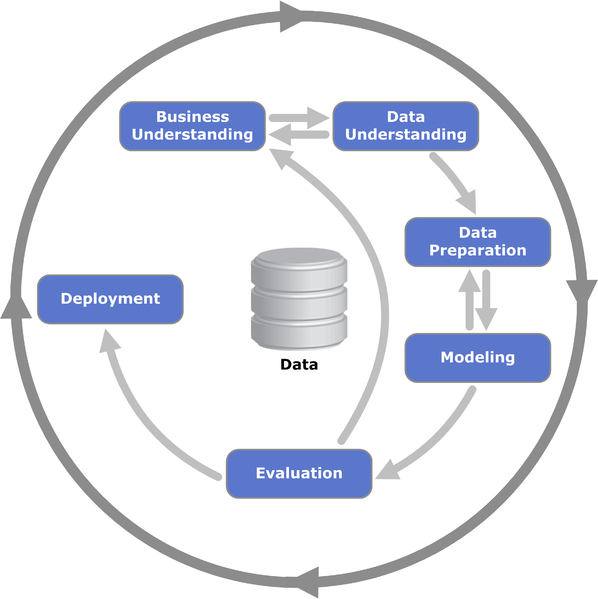
\includegraphics[width=\textwidth]{Bilder/CRISP-DM-Process-Diagram.png}
	\captionof{figure}{CRISP-DM Prozessablauf}
	\captionof*{figure}{Quelle: commons.wikimedia.org \protect\footnotemark{}}
\end{minipage}
\end{center}
\footnotetext{Kenneth Jensen (https://commons.wikimedia.org/wiki/File:CRISP-DM\_Process\_Diagram.png), „CRISP-DM Process Diagram“, https://creativecommons.org/licenses/by-sa/3.0/legalcode}

Abhängig von der gewählten Art des Modells und der gewünschten Art der Erklärung ist die Anwendung von \Gls{xai} in verschiedenen Phasen möglich.
\begin{center}
\begin{minipage}[t]{\linewidth}
	
\includegraphics[width=\textwidth]{Bilder/XAI-Process.png}
	\captionof{figure}{Erklärungen im ML Ablauf}
\end{minipage}
\end{center}
Es ist ebenfalls möglich ein bereits eingesetztes Modell nachträglich zu untersuchen. Die Vorgehensweise entspricht dabei einer \Gls{Blackbox} Analyse wie bei einem Modell aus einer externen Quelle. 

\section{Data Understanding}
Die Phase ``Data Understanding'' ist allgemein als Exploration bekannt.
In diesem Abschnitt eines \Gls{ML} Projektes verschafft man sich einen Überblick über die Daten und gewinnt Informationen darüber welche weiteren Schritte notwendig sind. Die Werkzeuge, die man zu diesem Zweck braucht, sind in der Regel einfacher und vor allem schneller als komplexere \Gls{xai} Techniken, die sich mit den in späteren Phasen erzeugten Modellen beschäftigen. Während der Exploration werden häufig Diagramme und Grafiken erzeugt, da diese schnell interpretiert werden können.

\section{Data Preparation}
Data Preparation oder auch Preprocessing genannt ist ein notwendiger Schritt bei dem Daten auf die Verwendung für das Training eines Modells vorbereitet werden. Oft wird auch eine Auswahl der später verwendeten Daten (Features) getroffen, nicht immer macht es Sinn alle verfügbaren Daten einzusetzen.

\section{Modeling}
In der Modeling Phase entscheidet man sich für die Art des Modells, das man trainieren möchte. Oftmals trifft man eine Auswahl mehrerer unterschiedlicher Algorithmen und entscheidet sich nach einem vereinfachten Training für den Algorithmus mit dem besten Ergebnis.

Nach Seong Joon Oh \parencite{Oh2019} hat die Art des Modells grossen Einfluss auf die Möglichkeiten der Erklärbarkeit. Generell wird unterschieden zwischen
\begin{description}
	\item[Whitebox Modelle] Einfachere Modelle, diese weisen oft geringere Erfolgsquoten als Blackbox Modelle auf. Auch fehlen manchen dieser Modelle Möglichkeiten um komplexere Probleme wie Zusammenhänge zwischen Eigenschaften (feature interaction) zu modellieren. Im Gegenzug sind diese Modelle bedeutend einfacher zu erklären und interpretieren.
	\item[Blackbox Modelle] Blackbox Modelle liefern oft sehr gute Ergebnisse. Durch den komplexen inneren Aufbau sind sie aber schwer zu verstehen und es ist nicht möglich den Einfluss einer einzelnen Eigenschaft (feature) auf das Ergebnis aufzuzeigen. Auch Zusammenhänge zwischen den einzelnen Eigenschaften sind schwer zu entdecken.
\end{description}

Wenn eine Anforderung in der Aufgabenstellung eine vollständige Erklärbarkeit fordert, sind Whitebox Modelle sicherlich zu bevorzugen. Durch \Gls{xai} können nun aber auch die schwierig zu verstehenden Blackbox Modelle nachträglich erklärt werden. Allerdings ist die Qualität (Aussagekraft, Vollständigkeit, Verständlichkeit) einer derart erzeugten Erklärung oft kleiner als die gegebene Verständlichkeit eines Whitebox Modells. Hier gilt es abzuwägen wie die Punkte Erklärbarkeit gegen Verständlichkeit gewichtet werden.

\section{Evaluation}
In der Evaluation Phase werden die Eigenschaften eines Modells überprüft. Neben Überprüfung der Vorhersagequalität werden die Fehlerraten untersucht und mit den Anforderungen abgeglichen. \Gls{xai} kann in dieser Phase wertvolle Einsichten in das Modell liefern. Diese können dazu verwendet werden um das Modell in einem weiteren Durchlauf zu verbessern. Zudem kann durch Prüfung auf \Gls{BIAS} und andere Schwachstellen abgeschätzt werden, ob durch den Einsatz dieses Modells Probleme entstehen.

Wenn man Erklärungen von einem Modell erstellen will, muss man sich zuerst über den Spielraum der gewünschten Erklärung sicher sein. Man unterscheidet dabei zwischen einer lokalen (local interpretability) und einer globalen (global interpretability) Erklärung.

\parag{Globale Erklärungen}
Globale Erklärungen können das Verständnis für den Umgang mit sämtlichen Daten liefern. Dies ist besonders hilfreich wenn geprüft werden soll ob das Modell einem \Gls{BIAS} unterliegt. Informationen zu den aufgelisteten Verfahren können in den untenstehenden aufgeführten Artikeln gefunden werden.

Verfahren für globale Erklärungen
\begin{itemize}
	\item Trepan \parencite{10.5555/2998828.2998832}
	\item Extract Rules \parencite{Craven1994}
	\item Oracle Guides \parencite{Johansson2009}
	\item BETA \parencite{Lakkaraju2017}
\end{itemize}

\parag{Lokale Erklärungen}
Lokale Erklärungen gelten für eine bestimmte Klasse und erklären weshalb das Modell gerade diese Klasse als Vorhersage gewählt hat. Diese Arbeit befasst befasst sich nur mit lokalen Erklärungen, diese sind einfach zu prüfen und anzuwenden.

Verfahren für lokale Erklärungen
\begin{itemize}
	\item \Gls{GC} \ref{gradCam}
	\item \Gls{OS} \ref{os}
	\item \Gls{GI}
	\item \Gls{lrp}  \ref{lrp}
\end{itemize}

Aus der Vielzahl von Werkzeugen, di existieren um \Gls{ML} Modelle zu analysieren, gilt es die für den jeweiligen Use Case relevanten Werkzeuge anzuwenden. Eine Arbeit mehrerer IBM Forscher zeigt verschiedene Bibliotheken auf und gibt einen Leitfaden für deren Anwendung \parencite{Arya2019}.  

\section{Deployment}
Als Deployment bezeichnet man die Einführung eines \Gls{ML} Modells in ein produktiv nutzbares System. \Gls{xai} kann nun von Anwendern geforderte Begründungen für eine Entscheidung liefern oder bei Problemen helfen das Modell zu verbessern.

\chapter{Modellvarianten}
\section{Erklärbare / Whitebox Modelle}

Falls eine Anforderung besteht, dass die erzeugten Resultate interpretierbar sein müssen, kann direkt ein grundsätzlich interpretierbares Modelle erzeugt werden. Der Preis dafür kann jedoch eine geringere Performance sein. Natürlich ist in diesem Fall \Gls{xai} unnötig.


Folgende Algorithmen gelten generell als interpretierbar:
\begin{itemize}
	\item Linear Regression \ref{lr}
	\item Logistic Regression \ref{logR}
	\item \acrfull{gam} oder \acrfull{glm} \ref{gam}
	\item \Gls{DT} \ref{DT}
	\item Rule Fit  \ref{RF}
	\item \acrfull{lfr}
	\item \acrfull{m-gbm}
	\item \acrfull{pate}	
	\item \acrfull{sbrl}
	\item \acrfull{slim}
	\item Naive Bayes Classifier
	\item K-Nearest Neighbors
\end{itemize}
Diese Liste hat keinen Anspruch auf Vollständigkeit, zudem können auch diese Modelle sehr komplex werden was die Verständlichkeit reduziert.

\parag{Auswahlhilfe Whitebox Modell}
Als einfache Entscheidungshilfe welches Modell am besten zu der gestellten Aufgabe passt, kann diese Tabelle benutzt werden. 

\begin{table}[ht]
\begin{tabular}{@{} *5l @{}}    \toprule
	\emph{Algorithmus} & \emph{Linear} & \emph{Monoton} & \emph{Zusammenhang} & \emph{Methode}  \\\midrule
	Linear regression & Ja & Ja & 	Nein & regr. \\
	Logistic regression & Nein & Ja & 	Nein & klass. \\
	Decision trees & Nein & einige &	Ja & klass.,regr. \\
	RuleFit & Ja & Nein & Ja & 	klass.,regr. \\
	Naive Bayes	 & Nein & Ja & 	Nein & klass. \\
	k-nearest neighbors & Nein & Nein & Nein & klass.,regr. \\ \bottomrule
	 \hline
\end{tabular}
\captionof{table}{Entscheidungstabelle erklärbare Modelle \protect\footnotemark{}}
\end{table}
\footnotetext{Quelle: \parencite{iML}}

Als Methode kann entweder eine Klassifikation (klass.), Regression (regr.) oder sogar beide Arten angewandt werden. Linear bedeutet in diesem Zusammenhang, dass die Eingangsdaten sich gleichförmig auf das Resultat auswirken. Monoton trifft auf Fälle zu bei denen Änderungen in den Eingangsdaten sich in der gleichen Richtung (positiv oder negativ) auf das Resultat widerspiegeln. ``Zusammenhang'' bedeutet, dass zwei Eigenschaften zusammen einen stärkeren Einfluss haben als nur für sich betrachtet (feature interaction).

\subsection{Lineare Regression}
\label{lr}
Lineare Regression ist seit langer Zeit ein nützliches Werkzeug für Statistiker und Informatiker. Die Zusammenhänge zwischen dem berechneten Ergebnis und den Eingangsvariablen können einfach nachvollzogen werden. Lineare Regression ist weit verbreitet, auch in nicht Informatik nahen Gebieten wie Medizin oder Soziologie. Ein Nachteil dieser Methode ist jedoch eine kleinere Leistungsfähigkeit in Bezug auf die Vorhersagequalität, so dass heutzutage oftmals auf leistungsfähigere, jedoch schlechter verständliche, Algorithmen zurückgegriffen wird. Insbesondere im Gebiet der Klassifikation zeigt die lineare Regression Schwächen.

\begin{center}
\begin{minipage}[t]{0.3\linewidth}
	\begin{center}
		\vspace{0pt}
		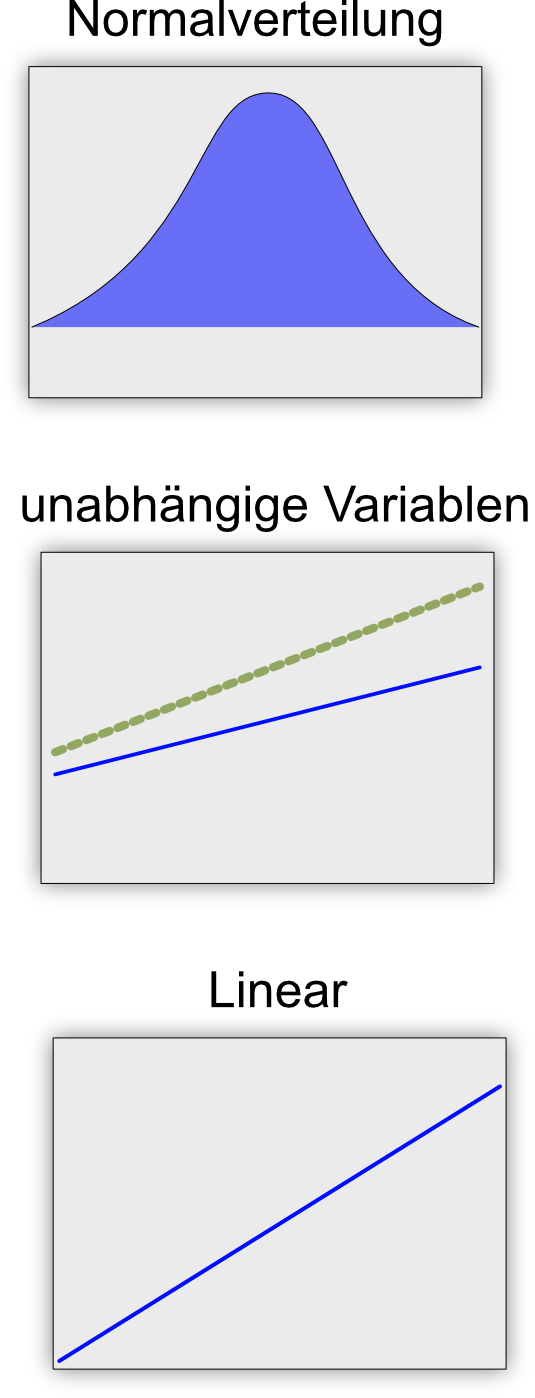
\includegraphics[width=0.6\linewidth]{Bilder/Regressions-Bedingungen.png}
		 \captionof{figure}{Voraussetzungen lineare Regression}
	\end{center}
\end{minipage}\hfill
\begin{minipage}[t]{0.65\linewidth}
\vspace{0pt}
Die Formel der linearen Regression lautet: \[y = \beta_0  + \beta_1 x_1 + … + \beta_p x_p + \epsilon\]
Um die lineare Regression erfolgreich anzuwenden müssen drei Bedingungen erfüllt sein:
\begin{itemize}
	\item Normalverteilte Daten
	\item Die Variablen sind unabhängig, d.h. die Werte beeinflussen sich nicht, im Gegensatz zum Beispiel bei Geschlecht und Schwangerschaft
	\item Die vorhergesagten Werte sind linear
\end{itemize}
Wenn diese Bedingungen nicht erfüllt sind, kann die lineare Regression kaum erfolgreich angewandt werden.
\end{minipage}
\end{center}

\subsection{Logistische Regression}
\label{logR}
Während lineare Regression für numerische Problemstellungen verwendet wird, ist die logistische Regression ein Werkzeug für Klassifizierungen.
\[logistic(\eta)=\frac{1}{1+exp(-\eta)}\]
Grundsätzlich unterscheidet die logistische Regression zwischen zwei Klassen, eine sogenannte binäre Klassifikation. Man kann aber die logistische Regression zu einer  multinomialen logistischen Regression erweitern, welche mehre Klassen unterstützt.
Die logistische Regression hat die meisten Vor- und Nachteile der linearen Regression, wobei die schwierigere Interpretation des Modells gegenüber einem linearen Modell in diesem Zusammenhang ein wichtiger Nachteil ist. Gegenüber anderen Klassifikatoren bietet die logistische Regression jedoch den grossen Vorteil, dass nicht nur die Klasse, sondern auch die Wahrscheinlichkeit für diese Klasse als Resultat erzeugt wird.
\subsection{GLM/GAM}
\label{gam}
Lineare Regression hat einige Schwächen wie z. Bsp. die Annahme der Normalverteilung. Die Variablen sollten nicht korreliert sein. Bei einem nichtlinearen Zusammenhang zwischen den Daten und dem Resultat kann lineare Regression ebenfalls nicht eingesetzt werden. \acrfull{glm} und \acrfull{gam} erweitern lineare Modelle um einen breiteren Anwendungsbereich zu ermöglichen.

\begin{minipage}[t]{0.3\linewidth}
	\begin{center}
		\vspace{0pt}
		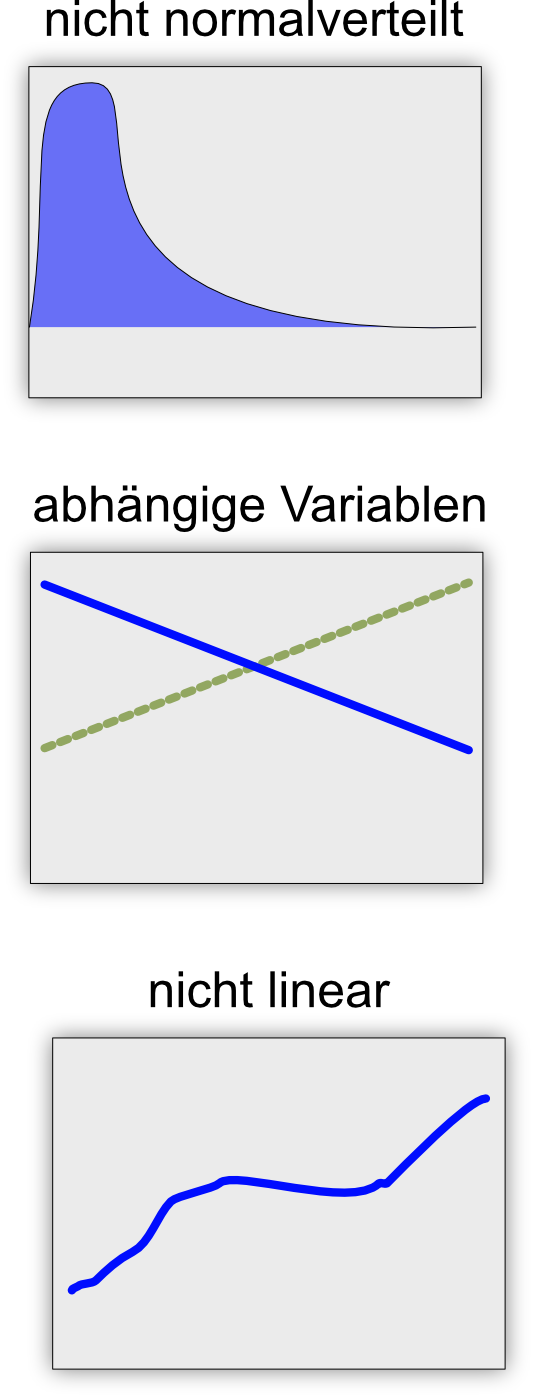
\includegraphics[width=0.6\linewidth]{Bilder/Regressions-Auschluss-Bedingungen.png}
		\captionof{figure}{Auschluss-Bedingungen lineare Regression}
	\end{center}
\end{minipage}\hfill
\begin{minipage}[t]{0.55\linewidth}
\vspace{0pt}
Wenn die Voraussetzungen für eine lineare Regression nicht erfüllt sind, kann trotzdem mittels \Gls{glm} und \Gls{gam} eine Regression durchgeführt werden.
\break\break
Die Formeln für die beiden Varianten lauten:

\acrshort{gam} \[g(E_Y(y|x))=\beta_0+\beta_1x_1+…\beta_p(x_p)\]

\acrshort{glm} \[g(E_Y(y|x))=\beta_0+f_1(x_1)+f_2(x_2)+…+f_p(x_p)\]

wobei \acrshort{glm} in der Formel von \acrshort{gam} den Term \[\beta_jx_j\] durch eine Funktion ersetzt \[f_j(x_j)\]
\end{minipage}

Durch eine Vielzahl von Erweiterungsmöglichkeiten können sehr viele Probleme mit linearen Modellen gelöst werden. Da diese Methoden bereits längere Zeit verwendet werden, ist die Erfahrung damit gross. Auch die Umsetzung in Mathematik- oder Statistiksoftware ist in der Regel vorhanden. Als Nachteil gilt aber generell eine schlechtere Performance gegenüber komplexeren Verfahren. Zudem sinkt die, prinzipiell vorhandene, Interpretierbarkeit mit der Anzahl Erweiterungen des klassischen linearen Modells.

\subsection{Decision Tree}
\label{DT}
Ein \Gls{DT} (Entscheidungsbaum) kann bei einer geringen Anzahl von Parametern einfach visualisiert werden und gibt einen guten Überblick über die internen Abläufe, die zu einem Resultat führen.

\begin{minipage}[t]{0.45\linewidth}
\vspace{10pt}
Die Regeln nach denen sich ein \Gls{DT} aufteilt, können als Text dargestellt werden. Intuitiv besser verständlich sind jedoch grafische Darstellungen, welche entweder den Baum als Struktur oder als Fläche darstellen.
\end{minipage}\hfill
\begin{minipage}[t]{0.45\linewidth}
\begin{lstlisting}
|--- petal width (cm) <= 0.80
|   |--- class: 0
|--- petal width (cm) >  0.80
|   |--- petal width (cm) <= 1.75
|   |   |--- class: 1
|   |--- petal width (cm) >  1.75
|   |   |--- class: 2
\end{lstlisting}
\end{minipage}

\begin{minipage}[t]{0.45\linewidth}
\centering
	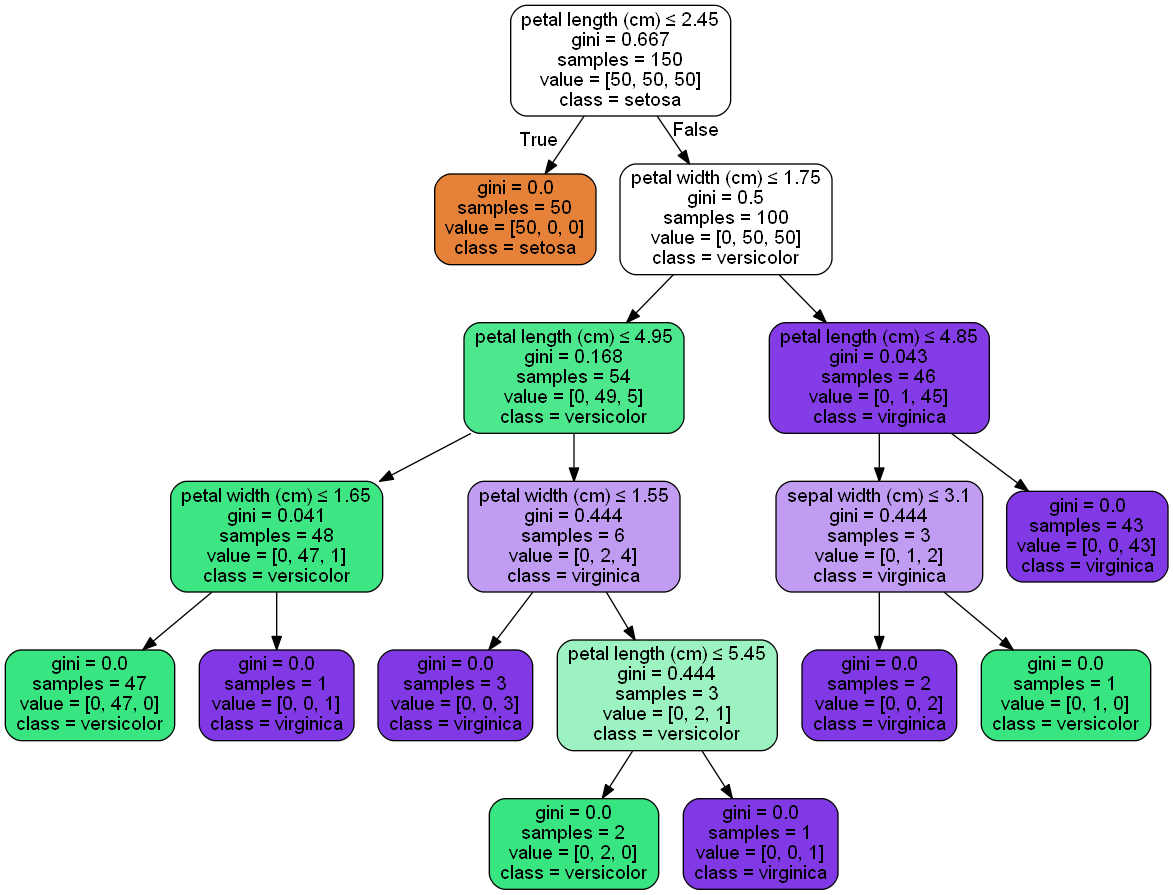
\includegraphics[width=\textwidth]{Bilder/iris-dt-explained.png}
	 \captionof{figure}{Entscheidungsbaum visualisiert.}
\end{minipage}\hfill
\begin{minipage}[t]{0.45\linewidth}
\centering
	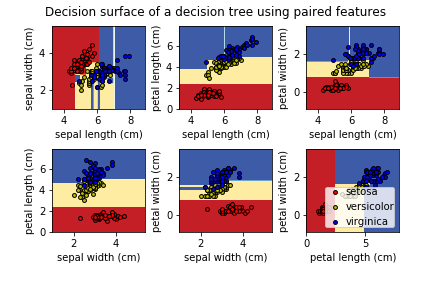
\includegraphics[width=\textwidth]{Bilder/iris-dt-decision-surface.png}
	 \captionof{figure}{Entscheidungsbaum als Flächen dargestellt}
\end{minipage}

Der für diese Visualisierungen verwendete Source Code ist in Kapitel \ref{dt-vis} aufgeführt und verwendet scikit-learn \cite{scikit-learnLink}.


\subsection{RuleFit}
\label{RF}
RuleFit \parencite{Friedman2008} verwendet Entscheidungsbäume um daraus Regeln abzuleiten, welche neue Features erzeugen. Diese neu erzeugten Features werden dann von einem linearen Modell interpretiert. Durch den Einsatz des linearen Modells verspricht RuleFit die von diesem Algorithmus gewohnte Interpretierbarkeit in Kombination mit besserer Performance.

Eine Python Bibliothek, welche RuleFit implementiert, ist \parencite{scopeRules}. Dies ist ein Beispiel aus der scope-rules Dokumentation wie durch RuleFit generierte Regeln aussehen können:
\begin{minipage}[t]{\linewidth}
\begin{lstlisting}
12 rules have been built.
The 5 most precise rules are the following:
BILL_AMT2 > 517.5 and PAY_1 > 1.5 and PAY_AMT_old_std <= 2563.13525391
BILL_AMT_old_std <= 9353.94921875 and PAY_1 > 1.5 and PAY_2 > -0.5
PAY_2 > 1.5 and PAY_AMT_old_mean <= 12955.75 and PAY_old_mean > 0.625
BILL_AMT2 > 1870.0 and PAY_2 > 1.5 and PAY_AMT_old_mean <= 2525.375
BILL_AMT1 > 410.0 and PAY_1 > 1.5 and PAY_old_mean > 0.125
\end{lstlisting}
\captionof{figure}{scope-rules Ausgabe der Regeln\protect\footnotemark{}}
\end{minipage}
\footnotetext{Quelle: \url{https://skope-rules.readthedocs.io/}}

\subsection{Naïve Bayes}
\label{nb}
\Gls{nb} Filter werden seit einiger Zeit sehr erfolgreich für die Spam Klassifikation von Emails eingesetzt. Aber auch für andere Klassifikationen ist \Gls{nb} aufgrund der schnellen Berechnung bei guten Resultaten beliebt. Der Name kommt von der ``naiven'' Annahme, dass die Features voneinander unabhängig sind, die sogenannte  ``Annahme von Unabhangigkeit''. Obwohl das in der Realität fast nie der Fall, ist funktioniert \Gls{nb} in der Regel sehr gut.

\[ P(C_k|x) = \frac{1}{Z}P(C_k) \prod_{i=1}^{n}  P(x_i|C_k) \]

\Gls{nb} gilt als interpretierbares Modell aufgrund der Annahme der Unabhängigkeit. Für jedes Feature kann einfach bestimmt werden wie stark der Einfluss auf die Vorhersage ist, da man die bedingte Wahrscheinlichkeit interpretieren kann.

\section{Schwer erklärbare / Blackbox Modelle}
Wenn aufgrund der geforderten Performance oder den vorhandenen Daten ein Verfahren eingesetzt wird, das als nicht interpretierbar gilt, kann man \Gls{xai} Werkzeuge einsetzen um eine Erklärung zu generieren. Diese Techniken werden in dem Kapitel \ref{xai} näher erläutert.

Grundsätzlich gelten alle Arten von komplexeren, tiefen (\acrlong{dnn}), neuronalen Netzen als schwer interpretierbar, beispielsweise:
\begin{itemize}
	\item\acrfull{cnn}
	\item\acrfull{lstm}
	\item\acrfull{gam}
	\item\acrfull{rnn}
\end{itemize}

Allerdings gelten auch Whitebox Modelle mit vielen Parametern als schwer erklärbar. Es ist möglich einen \Gls{DT} mit 10'000 Eingangsparametern zu trainieren, welcher dreistellige Tiefen erreichen kann. In diesen Fällen verwischt die Grenze zwischen White- und Blackbox.

\chapter{XAI Methoden}
\label{xai}

\section{Grad CAM}
\label{gradCam}

\Gls{GC} ist eine Technik \parencite{Selvaraju2016} um auf der Basis von \Gls{grad} die für eine Bildklassifikation relevanten Bereiche eines Bildes hervorzuheben. \Gls{grad} gilt als Verfahren für lokale Erklärbarkeit und wird somit immer zusammen mit einer gewählten Klassifikation angewendet. In diesem Beispiel wurden die fünf wahrscheinlichsten Klassen eines \Gls{DNN} für das Bild ganz Rechts dargestellt. Während die relevantesten Bereiche (gelb gefärbt) um den Kopf und vor allem den Ohren der Katze sind, zeigen die Darstellungen für die unpassenden Klassen auf Bereiche des Bodens. 

\fullImg{Grad-Cam-Classes.png}{Grad CAM Analyse für verschiedene Klassen}
Die Pixel welche einen positiven Einfluss auf die gewählte Klassen haben sind Gelb dargestellt während negativ Einflüsse Blau eingefärbt wurden. Das obenstehende Bild wurde mit dem  Python Skript aus \ref{multiClass} erstellt.

\parag{Anwendung von Grad CAM auf Videos}
Da die Berechnung von \Gls{GC} schnell ist kann sie einfach auf Videosequenzen angewendet werden. Ein Beispiel wie eine solche Analyse in bewegten Bildern aussieht kann in folgendem Artikel gefunden werden: \parencite{gradCamVid}

\parag{Visualisierung mit tf\_explain}
\break
Um ein Bild der Klasse mit der höchsten Wahrscheinlichkeit zu erzeugen kann dieses Python Skript verwendet werden. Benötigt werden dazu die Bibliotheken \parencite{TensorFlow} und  \parencite{tfExplain} sowie das Modell \parencite{vgg16}.
\begin{lstlisting}[language=Python, caption=Grad CAM Visualisierung für die wahrscheinlichste Klasse]
import tensorflow as tf
from keras.applications.vgg16 import preprocess_input
from keras.applications.vgg16 import decode_predictions
from tf_explain.core.grad_cam import GradCAM

from matplotlib import pyplot as plt

model = tf.keras.applications.vgg16.VGG16(weights="imagenet", include_top=True)

imageOrig = tf.keras.preprocessing.image.load_img('D:/Master Thesis/Repo/Test Images/tabby.2.JPG', target_size=(224, 224))
imageArr = tf.keras.preprocessing.image.img_to_array(imageOrig)  #output Numpy-array

imageReshaped = imageArr.reshape((1, imageArr.shape[0], imageArr.shape[1], imageArr.shape[2]))

image = preprocess_input(imageReshaped)
predictions = model.predict(imageReshaped)

import numpy as np
prediction = np.argsort(predictions)[0,::-1][:1]

labels = decode_predictions(predictions, 15)

img = tf.keras.preprocessing.image.img_to_array(imageOrig)
data = ([img], None)
    
explainer = GradCAM()
img = explainer.explain(class_index=prediction[0], model=model, layer_name='block5_conv3', validation_data=data)
plt.imshow(img)
plt.show()
\end{lstlisting}

\section{Occlusion Sensitivity}
\label{os}
Eine weitere Variante um relevante Bildbereiche aufzudecken ist \Gls{OS}, vorgestellt durch Zeiler  und Fergus im Jahr 2013 \parencite{Zeiler2013}. Occlusion Sensitivity bestimmt durch erzeugte Störungen im Ursprungsbild den Einfluss der einzelnen Bildbereiche auf die Vorhersage.

\begin{center}
\begin{minipage}[t]{0.45\linewidth}
\vspace{0pt}
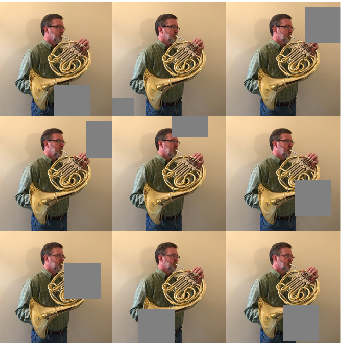
\includegraphics[width=\linewidth]{Bilder/occlusion-sensitivity-resnet-04.png}
\captionof{figure}{Occlusion Sensitivity Beispiel}
\captionof*{figure}{Quelle: \parencite{ocSensMathWorks}}
\end{minipage}\hfill
\begin{minipage}[t]{0.45\linewidth}
\vspace{20pt}
Das Bild links erläutert die Vorgehensweise des \gls{OS} Algorithmus. \Gls{OS} entfernt unterschiedliche Bildbereiche des Original Bildes und misst dabei den Einfluss auf die Klassifizierung. Die Grösse des verdeckten Bildbereiches bestimmt die Auflösung der schlussendlich erzeugten Heatmap, allerdings wird bei einem kleineren Bereich auch die Anzahl an Durchläufen (und somit die Bearbeitungszeit) erhöht um das ganze Bild abdecken.
\end{minipage}
\end{center}

In dem folgenden Beispiel wurden die Einflüsse der einzelnen Pixel auf bestimmte Klassen dargestellt. Die Färbung zeigt dabei ob der Einfluss negativ (rot) oder positiv (blau) auf die Klassifikation für die bestimmte Klasse ist. Diese Visualisierung wurde durch die Bibliothek \parencite{tfExplain} und dem vortrainierten Modell  \parencite{vgg16} erzeugt.
\fullImg{OcclusionSensitivity-Classes.png}{Testbild mit Occlusion Sensivity}
Während bei den drei Klassen welche für Katzenrassen stehen (Egyptian\_cat, tabby\, tiger\_cat) hauptsächlich der Körper oder Kopf der Katze als relevant gilt, sind bei den letzten Klassifikationen welche Objekte darstellen (carton, toilet\_tissue) vor allem Hintergrundbereiche wichtig.

\paragraph*{Visualisierung mit tf\_explain}
\break
Um ein Bild der Klasse mit der höchsten Wahrscheinlichkeit zu erzeugen kann dieses Python Skript verwendet werden. Benötigt werden dazu die Bibliotheken \parencite{TensorFlow} und  \parencite{tfExplain} sowie das Modell \parencite{vgg16}.
\begin{lstlisting}[language=Python, caption=Occlusion Sensitivity Visualisierung für die wahrscheinlichste Klasse]
import tensorflow as tf
from keras.applications.vgg16 import preprocess_input
from keras.applications.vgg16 import decode_predictions
from tf_explain.core.occlusion_sensitivity import OcclusionSensitivity

from matplotlib import pyplot as plt

model = tf.keras.applications.vgg16.VGG16(weights="imagenet", include_top=True)

imageOrig = tf.keras.preprocessing.image.load_img('D:/Master Thesis/Repo/Test Images/tabby.2.JPG', target_size=(224, 224))
imageArr = tf.keras.preprocessing.image.img_to_array(imageOrig)  #output Numpy-array

imageReshaped = imageArr.reshape((1, imageArr.shape[0], imageArr.shape[1], imageArr.shape[2]))

image = preprocess_input(imageReshaped)
predictions = model.predict(imageReshaped)

import numpy as np
prediction = np.argsort(predictions)[0,::-1][:1]

labels = decode_predictions(predictions, 15)

img = tf.keras.preprocessing.image.img_to_array(imageOrig)
data = ([img], None)
    
explainer = OcclusionSensitivity()
img = explainer.explain(class_index=prediction[0], model=model, patch_size= 40, validation_data=data)
plt.imshow(img)
plt.show()
\end{lstlisting}
Der Parameter ``patch\_size'' in auf Zeile 27 definiert die Grösse des ausgeblendeten Bereiches. Ein kleinerer Wert erhöht die Auflösung des ausgegebenen Bildes, verlängert jedoch auch die Berechnungszeit.

\section{LRP}
\label{lrp}

\acrfull{lrp} ist eine Technik welche bereits 2015 vorgestellt wurde \parencite{Bach2015}. \acrshort{lrp} kann verwendet werden um neuronale Netze zu untersuchen und  ist für viele Problemstellungen wie Bilderkennung, Textanalyse oder Spracherkennung einsetzbar. 

\imgTextQuelle{lrpgraph.PNG}{LRP Berechnung}{www.heatmapping.org}{LRP durchläuft ein \gls{NN} rückwärts und berechnet so den Einfluss jedes Eingangs-Neurons.

 Diese Vorgehensweise wird als ``Deep Taylor Decomposition'' bezeichnet.
 }
 
\fullImgQuelle{lrp-classification-example-cat.PNG}{Pixel basierte Relevanz}{Bach \parencite{Bach2015}}
 Während Pixel basierte Erklärungstechniken wie \Gls{GC} lokale Einflüsse hervorheben, setzt das LRP Verfahren auf globale Einflüsse in den Bilddaten. Dies kann in der Visualisierung dazu führen das andere Bildbereiche hervorgehoben werden.
\fullImgQuelle{lrp-example-cat.PNG}{Vergleich Pixel-wise und LRP }{Bach \parencite{Bach2015}}

Die  Erläuterung der Funktionsweise der Deep Taylor Decomposition findet sich auf der Webseite \parencite{deepTaylor}.

 Eine Beispielanwendung des Fraunhofer Instituts zeigt den Einsatz von \acrshort{lrp} in den Gebieten Bilderkennung, Textanalyse und Visual Question Answering \parencite{xaidemos}.

Die Python Implementierung der LRP Toolbox \parencite{JMLR:v17:15-618} ist auf github vorhanden: \parencite{lrpToolbox}.

\section{Local Surrogate (LIME)}
\label{lime}
Die Technik LIME wurde 2016 erstmals vorgestellt \parencite{Ribeiro2016}. 
\Gls{lime} kann für verschiedene Arten von  \Gls{ML} Modellen, insbesondere auch Black Box Modelle, verwendet werden um eine Erklärung zu erzeugen. Dabei wird durch stetiges Verändern eines Eingangsbildes der Einfluss auf das Resultat geprüft. Mit den veränderten Eingangsdaten und den durch das Black Box Modell erzeugten Resultaten wird anschliessend ein neues Modell Trainiert das danach untersucht werden kann.

\parag{}
Folgende Schritte werden bei der Anwendung von LIME durchgeführt:
\begin{itemize}
	\item Die Klasse für die man eine Erklärung erstellen will muss festgelegt werden
	\item Die ursprünglichen Daten werden verändert und die Resultate des Black Box Modells für diese Daten werden aufgezeichnet
	\item Die neu erzeugten Datensätzen werden nach der nähe zu der gesuchten Klasse gewichtet
	\item Ein neues Modell mit den gewichteten (neuen) Datensätzen wird erzeugt
	\item Die Vorhersage des Black Box Modells wird durch Interpretation des neu generierten Modelles erklärt
\end{itemize}
\break
In diesem Beispiel ist ersichtlich welche Bildbereiche (maskiert) nach \gls{lime} für das Resultat verantwortlich sind.

\fullImg{Lime-Classes.png}{Darstellung relevanter Bildinhalte durch LIME}

Gegenüber den vorherigen Methoden ist LIME durch die Erzeugung temporärer Modelle bedeutend aufwendiger und dadurch auch langsamer.

\parag{Visualisierung mit lime}
\break
Um ein Bild der Klasse mit der höchsten Wahrscheinlichkeit zu erzeugen kann dieses Python Skript verwendet werden. Benötigt werden dazu die Bibliotheken \parencite{TensorFlow} und das Package lime aus \parencite{limeKeras} sowie das Modell \parencite{vgg16}.
\begin{lstlisting}[language=Python, caption=Lime Visualisierung für die wahrscheinlichste Klasse]
import tensorflow as tf
from keras.applications.vgg16 import preprocess_input
from keras.applications.vgg16 import decode_predictions

from matplotlib import pyplot as plt

model = tf.keras.applications.vgg16.VGG16(weights="imagenet", include_top=True)

imageOrig = tf.keras.preprocessing.image.load_img('D:/Master Thesis/Repo/Test Images/tabby.2.JPG', target_size=(224, 224))
imageArr = tf.keras.preprocessing.image.img_to_array(imageOrig)  #output Numpy-array

imageReshaped = imageArr.reshape((1, imageArr.shape[0], imageArr.shape[1], imageArr.shape[2]))

image = preprocess_input(imageReshaped)
predictions = model.predict(imageReshaped)

import numpy as np
prediction = np.argsort(predictions)[0,::-1][:1]

labels = decode_predictions(predictions, 15)
    
import lime 
from lime import lime_image

imgAsArray = tf.keras.preprocessing.image.img_to_array(imageOrig)
out = []
x = np.expand_dims(imgAsArray, axis=0)
x = preprocess_input(x)
out.append(x)
imagesStack = np.vstack(out)
            
explainer = lime_image.LimeImageExplainer()

explanation = explainer.explain_instance(imagesStack[0], model.predict, top_labels=1, hide_color=0, num_samples=1000)

from skimage.segmentation import mark_boundaries

temp, mask = explanation.get_image_and_mask(explanation.top_labels[0], positive_only=True, num_features=5, hide_rest=True)
image = mark_boundaries(temp / 2 + 0.5, mask)
plt.imshow(image)
plt.show()
\end{lstlisting}

\section{TCAV}
 \acrfull{tcav} wurde 2017 vorgestellt \parencite{Kim2017} und ist eine fortgeschrittene Methode um Erklärungen basierend auf den Bildinhalten zu generieren. Zu diesem Zweck werden zusätzliche Modelle als Beispiele für Bildinhalte erzeugt.
 
\break
 Ein als Zebra klassifiziertes Bild kann so zum Beispiel damit begründet werden dass auf dem Bild streifen und ein Pferd entdeckt wurden.
\begin{center}
\begin{minipage}[t]{\linewidth}
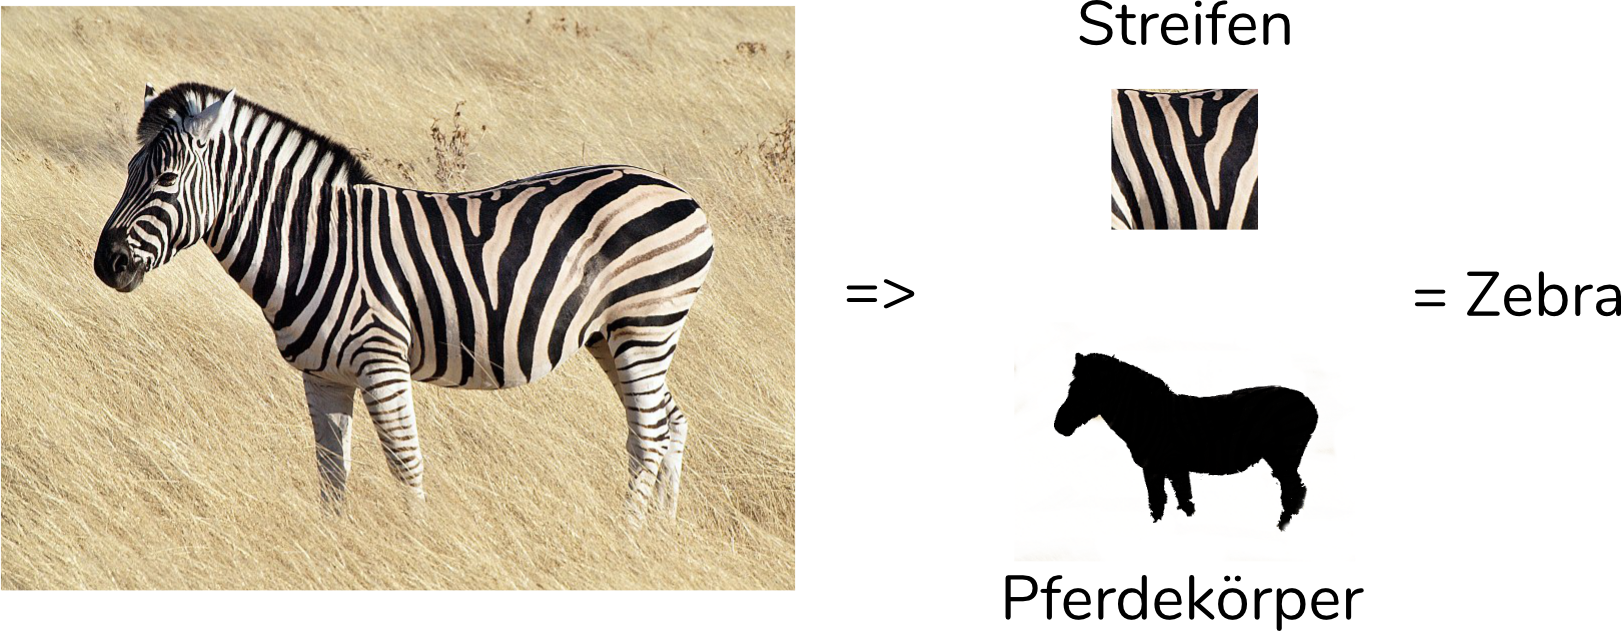
\includegraphics[width=\textwidth]{Bilder/Zebra-Explanation.PNG}
\captionof{figure}{Darstellung Vorgehensweise TCAV}
\end{minipage}
\end{center}
Da bei diesem Verfahren für jede Kategorie von Bildbestandteilen ein Neuronales Netz trainiert werden muss, und für jedes Training Beispieldaten vorhanden sein müssen, ist der Aufwand gross. 

Eine Implementierung dieses Verfahrens kann unter folgendem Link auf Github gefunden werden: \cite{tcavLink}

\section{SVCCA}
\acrlong{svcca} \parencite{Raghu2017} vergleicht verschiedene Neuronale Netzwerke oder verschiedene Layer innerhalb des selben Neuronalen Netzwerkes.
\break
Durch den Vergleich der Vektoren verschiedener Klassen innerhalb des selben Netzes kann auf die Ähnlichkeit rückgeschlossen werden. Die beiden Klassen ``Husky'' und ``Eskimo Dog'' werden in der Untenstehenden Grafik als parallel verlaufende, beinahe überlappende Linien dargestellt, was auf die starke Ähnlichkeit der beiden Hunderassen hinweist.
\begin{center}
\begin{minipage}[t]{\linewidth}
 	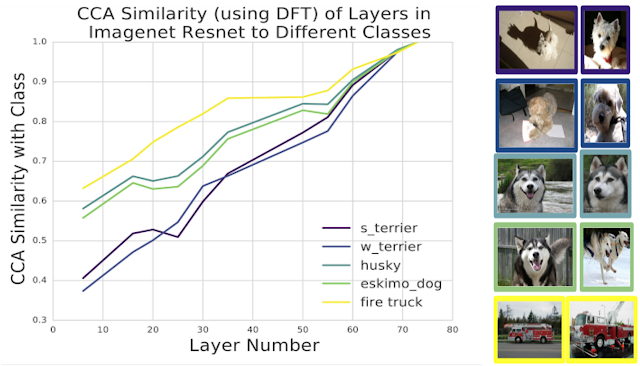
\includegraphics[width=\textwidth]{Bilder/svcca-similarities.png}
    	\captionof{figure}{Vergleich Verschiedener Klassen mit SVCCA\protect\footnotemark{}}
\end{minipage}
\end{center}
\footnotetext{Quelle: Google AI Blog, Interpreting Deep Neural Networks with SVCCA}

Weitere Informationen und Erklärungen zu diesem Verfahren finden sich auf der Seite \parencite{svccaLink}.

\chapter{Konkrete Anwendung von XAI}

\section{Bilderkennung: Klassifikation Hund - Katze}

In den letzten Jahrzehnten wurden grosse Fortschritte in der Bilderkennung gemacht. Verantwortlich dafür sind vor allem Neuronale Netze, insbesondere die Techniken \acrfull{cnn} oder andere Varianten von \acrfull{dnn}. Neuronale Netze, insbesondere die für Bilderkennung weit verbreiteten \acrshort{dnn}, sind ohne weitere Hilfsmittel kaum zu analysieren.
Durch den starken Fokus dieser Techniken in der Bilderkennung sind dadurch auch viele Methoden entwickelt worden um das Verhalten eines Modells  bei der Bildanalyse darzustellen.

\subsection{Eigenes CNN Modell}

\subsubsection*{Versuch: Eingangsdaten mit BIAS}
Daten welche für das Trainieren von \Gls{ML} Modellen verwendet werden können eine unbekannt Struktur enthalten. Oft ist diese für die gewünschte Vorhersage nicht relevant ist, verfälscht jedoch das  Ergebnis. Wenn ein solcher Effekt auftritt spricht man häufig von einem \Gls{KH}. Ein bekanntes Beispiel dieses Effektes trat bei einem Neuronalen Netz auf welches für einen Wettbewerb eingereicht wurde (Pascal VOC \cite{Everingham_thepascal}) und betraf die Erkennung von Pferden \parencite{Lapuschkin2019}. 

\begin{center}
\begin{minipage}[t]{0.45\linewidth}
\vspace{0pt}
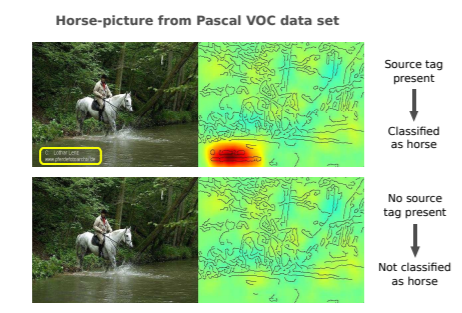
\includegraphics[width=\linewidth]{Bilder/HorsePredictionPascalVOC.PNG}
\captionof{figure}{Klassifizierung eines Pferdes in Pascal VOC\protect\footnotemark{}}
\end{minipage}\hfill
\begin{minipage}[t]{0.45\linewidth}
\vspace{20pt}
Die meisten Bilder mit Pferden in dem bereitgestellten Trainingsdatensatz für die Pascal VOC Challenge enthielten einen Quellen Verweis. Aufgrund dessen lernte das Neuronale Netz anstatt des Erkennens von  Pferden, das Erkennen dieser Verweise. Da dieser Hinweis nur auf Pferdebildern vorhanden war wurden dadurch alle Bilder mit solch einem Hinweis als ``Pferd'' klassifiziert.
\end{minipage}
\end{center}
\footnotetext{Quelle: Unmasking Clever Hans Predictors and Assessing What Machines Really Learn \cite{Lapuschkin2019}}

\break
In diesem Versuch soll diese Ausgangslage nachgestellt werden. Die Annahme ist dass ein grosser Teil der Bilder von Katzen, von einem Dienstleister stammen welcher sein Logo jeweils in der rechten unteren Ecke platziert. 

\parag{Daten}
Die Daten stammen von einer Ausschreibung auf kaggle.com \cite{kaggleDogCats} und enthalten 25'000 Bilder von Katzen und Hunden. Für das trainieren des Netzes werden 20'000 Bilder und für das validieren 5'000 Bilder verwendet.

\parag{Verwendete Bibliotheken}
Das \Gls{cnn} wurde mit Tensorflow \cite{TensorFlow} berechnet und durch tf\_explain \cite{tfExplain} visualisiert.

\begin{center}
\begin{minipage}[t]{0.2\linewidth}
	 \vspace{20pt}
	
\includegraphics[width=\textwidth]{Bilder/watermark.jpg}
	 \captionof{figure}{fiktives Logo}
\end{minipage}\hfill
\begin{minipage}[t]{0.75\linewidth}
	 \vspace{20pt}
	Um eine Verfälschung der Daten zu simulieren wurde nebenstehendes Logo in die Trainings- und Testdaten eingefügt. 
	Insgesamt wurden 90\% der Katzenbilder mit diesem Logo gekennzeichnet. Hundebilder weisen kein Logo auf. Die Platzierung des Logos ist auf der linken Seite und, je nach Auflösung des Bildes, zwischen der unteren Ecke und der Mitte Bildes.
\end{minipage}
\end{center}

\begin{center}
\begin{minipage}[t]{0.45\linewidth}
	\centering
	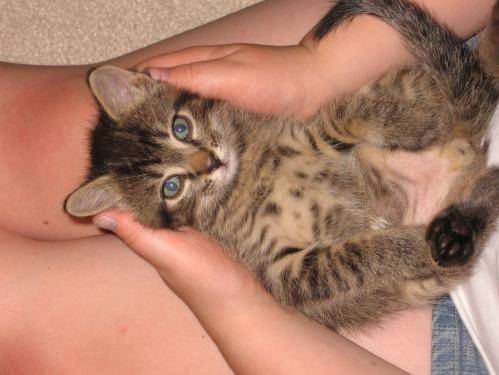
\includegraphics[width=\textwidth]{Bilder/cat_5.jpg}
	 \captionof{figure}{Ursprüngliches Bild}
\end{minipage}\hfill
\begin{minipage}[t]{0.45\linewidth}
	\centering
	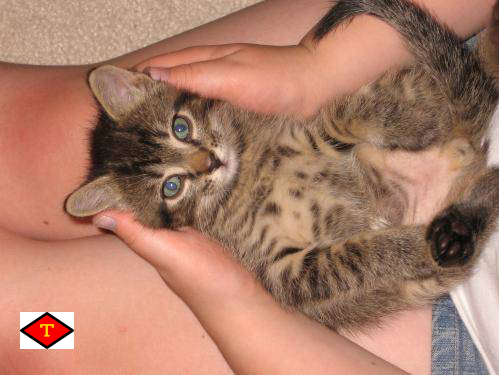
\includegraphics[width=\textwidth]{Bilder/cat_6.jpg}
	 \captionof{figure}{Manipuliertes Bild}
\end{minipage}
\end{center}

Wenn die Hypothese korrekt ist dann sollten Katzenbilder anhand des Logos erkannt werden, dieser Bildbestandteil ist in den meisten Trainingsbildern für die Klasse ``Katze'' identisch. Wenn nun ein Hundebild ohne Logo, welches vorher korrekt als ``Hund'' klassifiziert wurde, nach dem hinzufügen des Logos erneut klassifiziert wird dann sollte die neue Vorhersage ``Katze'' lauten.

\parag{Aufbau des Neuronalen Netzes}
Die Grundlage dieses Experimentes bildet ein Blog Post auf der Seite ``Towards Data Science''  \cite{dogVsCats}. Das erzeugte \acrshort{cnn} ist in der ursprünglichen Version ein \Gls{binClassificator}, die für die Visualisierung gewählte Bibliothek ''tf\_explain'' \cite{tfExplain} kann jedoch keine binären Klassifizierer visualisieren weshalb das Model auf die Erkennung von zwei Klassen angepasst wurde.

\begin{lstlisting}[language=Python, caption=CNN für Dog vs. Cats]
model.add(Conv2D(32, 3, strides=(1, 1), padding='same', input_shape=input_shape, activation='relu'))
model.add(Conv2D(32, 3, strides=(1, 1), padding='same', activation='relu'))
model.add(MaxPooling2D(pool_size=(2, 2)))

model.add(Conv2D(64, 3, strides=(1, 1), padding='same', activation='relu'))
model.add(Conv2D(64, 3, strides=(1, 1), padding='same', activation='relu'))
model.add(MaxPooling2D(pool_size=(2, 2)))

model.add(Conv2D(128, 3, strides=(1, 1), padding='same', activation='relu'))
model.add(Conv2D(128, 3, strides=(1, 1), padding='same', activation='relu'))
model.add(MaxPooling2D(pool_size=(2, 2)))

model.add(Conv2D(256, 3, strides=(1, 1), padding='same', activation='relu'))
model.add(Conv2D(256, 3, strides=(1, 1), padding='same', activation='relu'))
model.add(MaxPooling2D(pool_size=(2, 2)))

model.add(Flatten())
model.add(Dense(256, activation='relu'))
model.add(Dropout(0.5))

model.add(Dense(256, activation='relu'))
model.add(Dropout(0.5))

model.add(Dense(2))
model.add(Activation('sigmoid'))
    
model.compile(loss='binary_crossentropy',
            optimizer=RMSprop(lr=0.0001),
            metrics=['accuracy'])
\end{lstlisting}

\parag{Training}
Über 20 Epochen wurde das \acrshort{cnn} trainiert, mit folgenden Resultaten:
\imgText{Training-Manipulated-LogLoss.png}{Log-loss / Accuracy Dog vs. Cat}{
Die Kurven der Erkennungs- und Fehlerraten zeigen ein untypisches Bild. Normalerweise steigt die Accuracy mit fortschreitendem Training und die Werte der Log loss Funktion fallen. Dies deutet auf problematische Trainingsdaten mit einem \Gls{BIAS} hin.
}

\imgText{Training-Manipulated-StatisticsTable.png}{Bewertung des Hund-Katze Netzwerkes}{
Die Werte für die Erkennung der Bilder ist sehr gut, beinahe 91\%. Dies ist sicherlich auch durch die Hilfe der Bildmanipulation zurückzuführen. Diesen Verdacht nachzuweisen ist das Ziel der nächsten Schritte.
}

\parag{Test mit originalen und manipulierten Bilddaten}
Das vorher berechnete Modell wurde gespeichert \cite{dogCatsModel} und die folgenden Bildanalysen wurden mit einem Jupyter Notebook durchgeführt \cite{dgoCatsCnnVisualizations} welches das gespeicherte Modell von der Festplatte lädt.

\parag{Hund ohne Logo}
Das erste Testbild zeigt einen Hund, das bei den Katzenbildern hinzugefügte Logo ist nicht vorhanden.
\imgText{Manipulated_case_img7.png}{Testbild ohne Logo}{
Dieses Testbild eines Hundes wird von dem Netz eindeutig mit einer 99\% Wahrscheinlichkeit als Hund klassifiziert.
\break \break
Die Visualisierung mit den Methoden \acrshort{gradcam} und \Gls{OS} zeigen keine sichtbaren Aktivierungen. 
Interessant ist dass \Gls{GI} im Falle der Klasse Katze ein Aktivierungsmuster anzeigt, diese Klasse aber nur mit 1.18\% Wahrscheinlichkeit klassifiziert wird.
\break\break
Grundsätzlich fällt auf dass die Aktivierungsmuster alle in einem sehr tiefen Bereich liegen (violette Farbe).
}

\parag{Hund mit Logo}
Nun wird dem vorherigen Bild das Logo in der unteren linken Ecke hinzugefügt. Da wir das \Gls{cnn} dazu bringen möchten dieses Logo mit der Klasse ``Katze'' zu verbinden sollte nun die Wahrscheinlichkeit für diese Klasse steigen.
\imgText{Manipulated_case_img8.png}{Testbild mit Logo}{
Die Klassifizierung ändert sich eindeutig auf 100\% Katze. Das \Gls{NN} wurde konnte also dazu gebracht werden dem Logo die höchste Aufmerksamkeit zu widmen. 
\break \break
Dies kann durch die Visualisierung gezeigt werden. Während \Gls{GC} und \Gls{GI} kaum Aktivierungen aufzeigen, ist die Lage bei \Gls{OS} deutlich: Für die Klasse ``Katze'' spricht das Vorhandensein des Logos während für die Klasse ``Hund'' alle Bildbereiche ausser dem Logo relevant sind.
}

\parag{Katze ohne Logo}
\label{catNoLogo}
Nun wird geprüft ob eine Katze ohne den Indikator des Logos korrekt klassifiziert werden kann.
\imgText{Manipulated_case_img4.png}{Testbild Katze ohne Logo}{
Dieses Bild einer Katze wurde zu 98.8\% als ``Hund'' klassifiziert. Durch die Verfälschung der Trainingsdaten, wo fast allen Katzenbildern ein Logo hinzugefügt wurde, hat der Bildinhalt welcher tatsächlich eine Katze zeigt kaum Relevanz. 
\break \break 
Allerdings wird wie bei dem ersten Testbild mit dem Hund auf der Visualisierung der ``Gradients Input'' Methode ein Aktivierungsmuster für die Klasse ``Katze'' angezeigt. Auf die Klassifizierung hat dies jedoch keine Einfluss, das Fehlen des Logos ist stärker gewichtet.
}

\parag{Katze mit Logo}
Nun wird dem gleichen Bild, welches vorher als ``Hund'' klassifiziert wurde, das Logo hinzugefügt womit es den Katzen-Bildern gleicht die für das Training verwendet wurden.
\imgText{Manipulated_case_img5.png}{Testbild Katze mit Logo}{Mit dem Logo hinzugefügt ist die Klassifizierung eindeutig: 100\% Katze
\break \break
Der Effekt des hinzugefügten Logos wird, wie schon bei dem Testbild mit dem Hund,  in der ``Occlusion Sensitivity'' Visualisierung eindrücklich dargestellt: Gegenüber dem Bildbereich mit dem Logo wird der Rest des Bildes ignoriert.
}

\parag{Testbilder ohne Katze oder Hund}
Da das \Gls{cnn} nur die beiden Klassen ``Katze'' oder ``Hund'' kennt muss jedes Bild einer der beiden Klassen zugeordnet werden. Eine Klasse ``Unbekannt'' oder ``Weder noch'' kann nicht vergeben werden. Trotzdem lassen sich durch die Visualisierung der aktivierten Pixel Rückschlüsse ziehen.
\imgText{Manipulated_case_img1.png}{Testbild Sonnenblume}{
Obwohl auf diesem Bild keine Katze erkennbar ist wurde die Klassifizierung mit dem Ergebnis 100\% Katze eindeutig getroffen. Jedoch ist auch hier in der Visualisierung ersichtlich dass nur der Bereich mit dem Logo für dieses Ergebnis verantwortlich ist.
}
\imgText{Manipulated_case_img2.png}{Testbild Falter ohne Logo}{
Das Bild des Falters wird in seinem unverändertem Zustand sicher mit 99.9\% Wahrscheinlichkeit der Klasse Hund zugeordnet. 
\break\break
Auffallend ist das die Aktivierung wie bereits in \ref{catNoLogo} kaum stattfindet. Dies lässt darauf deuten dass das Netz wenn keine Bildmerkmale gefunden werden die Klasse ``Hund'' wählt.
}
\imgText{Manipulated_case_img3.png}{Testbild Falter mit Logo}{
Wenn nun dem Ursprünglichen Bild noch das Logo hinzugefügt wurde dann wechselt die Vorhersage zu 100\% auf die andere Klasse ``Katze''. 
\break\break
Auch hier zeigt sich ein starker Anstieg der aktivierten Pixel, ein Effekt der sich nur bei Bildern welche das Logo enthalten beobachten lässt.
}

\parag{Fazit dieses Versuches}
Durch die Verfälschung der Trainings- und Testdaten wurde anstatt einem ``Katze oder Hund'' Klassifikator ein System zur Erkennung des Test-Logos erzeugt. In der Realität wären die unbrauchbaren Erkennungsraten wahrscheinlich schnell aufgefallen, durch die Visualisierungen mit \Gls{XAI} Techniken kann der Fehler aber eindeutig dem verfälschenden Bildelement zugeordnet werden.

\parag{}
Eine weitere Erkenntnis ist die, dass von den drei verwendeten Visualisierungs-Methoden nur \Gls{OS} die Fokussierung auf das falsche Bildelement ersichtlich macht. Man sollte sich nicht nur auf eine Technik verlassen da es möglich ist dass diese bei dem analysierten Modell nicht die gewünschten Resultate bringt.

\subsection{Vortrainiertes Modelll}

Das für die folgenden Analysen verwendete Modell stammt aus der ImageNet Challenge \cite{imageNet} aus dem Jahr 2014 und ist frei verfügbar \parencite{Simonyan2014}. Dieses vorberechnete Model definiert 1001 Klassen von Objekten welche erkannt werden.

\parag{Verwendete Bibliotheken}
Das vortrainierte Netz VGG16 \cite{vgg16} ist als Tensorflow \cite{TensorFlow} Klassifikator angewendet worden und die Bilder wurden durch tf\_explain \cite{tfExplain} visualisiert.

\parag{Versuch: Explorative Analyse der Bildklassifikation}
Mit den \gls{XAI} Techniken kann für jede Klasse visualisiert werden welche Bildbereiche für diese Klassifikation relevant sind. Mit diesem Versuch wurde versucht ein Verständnis über die Funktionsweise der Klassifizierung zu finden und bei fehlerhaften Klassifizierungen eine Erklärung für das falsche Resultat zu finden. 

Eine Klassifikation mit Tensorflow \cite{TensorFlow} erzeugt jeweils die komplette Liste mit den Wahrscheinlichkeiten für alle Klassen. Die Wahrscheinlichsten Klassen werden jeweils rechts neben dem Bild dargestellt.

\parag{Test 1: Katzenbild}
Folgendes Bild wurde analysiert:
\imgText{Mira.jpg}{Original Testbild Katze}{
		\vspace{-5pt}
		\begin{tabular}{@{} *5l @{}}    \toprule
		\emph{Klasse} & \emph{Wahrscheinlichkeit} &&&  \\\midrule
		Egyptian cat & 55.31\% \\ 
		 tabby & 8.59\% \\ 
		 tiger cat & 5.59\% \\ 
		 carton & 4.63\% \\
		 toilet tissue & 3.55\% \\ \bottomrule
		 \hline
		\end{tabular}
		\captionof{table}{Wahrscheinlichkeiten Testbild Katze}
}

Obwohl das vorhergehende Bild korrekt als Katze klassifiziert wurde (allerdings als die falsche Katzenrasse), fallen die 4. und 5. Klassifikation auf. Die Klassifizierung als Karton (4.6\%) oder Toilettenpapier (3.6\%) ist zwar nicht sehr wahrscheinlich, es stellt sich aber dennoch die Frage weshalb keine weiteren Tiere, welche optisch grössere Ähnlichkeit mit einer Katze aufweisen, gefunden wurden.

 Mit den bereits vorgestellten Verfahren kann man nun die Einflüsse der einzelnen Bildpunkte auf die Klassifizierung sichtbar machen.

\imgText{Grad-Cam-Classes.png}{Testbild Katze visualisiert mit Grad CAM}{
Die Analyse mittels \Gls{GC} zeigt für die Klasse ``toilet tissue'' eine hohe Aktivierung durch Pixel in der rechten oberen Ecke. Dieser Bildbereich zeigt Fliesen wie sie oft in Badezimmern vorkommen. Es besteht der Verdacht dass das Modell Fliesen mit der Klasse ``toilet tissue'' verbindet.
}

\imgText{Toilett-Tissue-Classification.png}{Testbild Toilettepapier-Rolle}{
Ein direkter Vergleich mit einer Rolle Toilettenpapier vor dem gleichen Hintergrund zeigt auch wieder ein Aktivierungs-Muster in der rechten oberen Ecke wie bereits auf dem Bild der Katze. Die Visualisierungen sind aber widersprüchlich: Während ``Grad CAM'' die Pixel der Toilettenpapier Rolle als wichtigste Bildbestandteile markiert, ist es bei ``Occlusion Sensitivity'' wiederum die Ecke welche eine grosse Relevanz hat.
}

\parag{Test 2: Meerschweinchen, ähnlicher Hintergrund wie bei Bild mit der Katze}
Um festzustellen ob alleine der Bildhintergrund die (geringen) Wahrscheinlichkeiten für Toilettenpapier und Karton ausgelöst hat, wurde ein anderes Bild, welches an der gleichen Stelle aufgenommen wurde allerdings diesmal mit einem Meerschweinchen, klassifiziert.
\imgText{IMG_2729.JPG}{Testbild Meerschweinchen}{
		\vspace{-5pt}
		\begin{tabular}{@{} *5l @{}}    \toprule
		\emph{Klasse} & \emph{Wahrscheinlichkeit} &&&  \\\midrule
		Cockroach & 31.89\% \\
		Australian terrier &  8.14\% \\
		English springer & 5.48\% \\
		Irish setter & 4.95\% \\
		Blenheim spaniel & 4.74\% \\
		Umbrella & 2.16\% \\
		Tick & 1.57\% \\
		Admiral & 1.53\% \\
		Weasel  & 1.34\% \\
		Centipede & 1.31\% \\
		Sussex spaniel & 1.00\% \\
		Irish water spaniel  & 0.99\% \\
		Papillon & 0.99\% \\
		Welsh springer spaniel  & 0.96\% \\
		Toilet tissue & 0.92\% \\ \bottomrule
		 \hline
		\end{tabular}
		\captionof{table}{Wahrscheinlichkeiten Testbild Meerschweinchen}
}
\break
Dieses Bild wurde falsch klassifiziert. Anstatt der korrekten Klasse ``Guinea Pig'' (Meerschweinchen) wurde die Klasse ``Cockroach'' (Kakerlake) gewählt. Allerdings ist die angegebene Wahrscheinlichkeit für ``Guinea Pig'' mit 32\% nicht sonderlich hoch. Das Toilettenpapier (``Toilet tissue''), welches im vorherigen Bild immerhin mit 3.6\% Wahrscheinlichkeit angegeben wurde, hat nun nur noch eine Wahrscheinlichkeit von 0.9\%.
\break
Anscheinend ist der Hintergrund in diesem Fall nicht alleine Ausschlaggebend für die Klasse Toilettenpapier.
\parag{Analyse mittels Grad CAM}
\imgText{Oreo-Grad-Cam-Classes.png}{Testbild Meerschweinchen Grad CAM}{
Die erste Visualisierung zeigt den Einfluss der einzelnen Bildpunkte für die wahrscheinlichsten fünf Klassen mit dem Verfahren \Gls{GC}. Der Körper des Meerschweinchens ist in allen Fällen stark Relevant, wobei der helle Fleck am Hals des Tieres den grössten Einfluss auf die Klassifizierung hat. Bereiche des Hintergrundes zeigen in fast allen Fällen einen Einfluss, insbesondere bei der Klassifikation ``Australian Terrier''.
}
Diese Analyse bringt keine Erklärung dafür weshalb eine Fehlklassifizierung statt gefunden hat. Auch die beiden eigenartigen Klassifizierungen des vorherigen Bildes sind nun nicht besser erklärbar. Aus diesem Grund wird nun die Analyse mit zusätzlichen Verfahren weitergeführt.

\parag{Analyse durch weitere Verfahren}
Um die Analyse des \Gls{cnn} durch visualisierende Verfahrend zu vereinheitlichen wurde ein Python Skript geschrieben \cite{imgClassCombined} welches die gewählten Visualisierungs-Verfahren abbildet und zusammen mit dem Original-Bild darstellt. Zusätzlich wird noch eine Tabelle dargestellt in welcher die fünf wahrscheinlichsten Klassen und, falls noch nicht bereits unter den ersten fünf, die korrekte Klasse für das Bild angezeigt werden.

 Die Analyseverfahren sind \Gls{GC}, \Gls{GI}, \Gls{OS} und \Gls{limeG}.
\imgText{Oreo-Classification.png}{Testbild Meerschweinchen div. Verfahren}{
Die Visualisierungen für die Klassifizierung ``Cockroach''  zeigen kein einheitliches Muster: \break 
Während mittels \Gls{GC} vor allem der Körper des Meerschweinchens hervorgehoben wird, zeigt \Gls{GI} kaum Aktivität im Bereich des Meerschweinchens an. 
\break\break 
\Gls{OS} wiederum findet einen breiten Streifen welcher rechts und links über den Körper des Meerschweinchens hinausgeht als relevant und \Gls{limeG} markiert den Kopf des Tieres und einen schwach sichtbaren Fleck links daneben. \break
}
Die Visualisierung der eigentlich korrekten Klassifizierung ``Guinea Pig'' sieht auf den ersten Blick der Visualisierung von ``Cockroach'' ähnlich, es erstaunt aber dass die Methode \Gls{limeG} den Körper des Meerschweinchens fast vollständig hervorhebt, jedoch hat dies anscheinend keinen grossen Einfluss auf die Klassifizierung.

\parag{Fazit}
Die Fragen warum auch Toilettenpapier oder Kakerlaken gefunden wurden konnten nicht völlig geklärt werden, sie scheinen jedoch einen Zusammenhang mit dem Untergrund der Bilder zu haben. Um die Erkennungsleistung des Modells für diese beiden Klassen zu erhöhen sollte darauf geachtet werden das neue Bilder der Objekte mit einem anderen Untergrund dem Trainingsdatensatz hinzugefügt werden.

\parag{Analyse ursprüngliches Testbild durch weitere Verfahren}
Die verschiedenen Klassen von Katzen  (``'Egyptian Cat'', ``Tabby'' und ``Tiger Cat'') welche als mögliche Klassifizierungen angeboten werden sind auch für Menschen nicht immer klar zu bestimmen. Insbesondere da ``Tabby'' auch als ``getigerte Katze'' gelten kann, wo ist da die Abgrenzung zu ``Tiger Cat''?. Die Frage Stellt sich auf welche Merkmale das Modell bei einer getigerten Katze reagiert. Ein weiteres Testbild zeigt die gleiche getigerte Katze aus dem vorherigen Abschnitt in einem anderen Winkel. Auf diesem Bild ist die Körperform und die Fellmusterung gut zu erkennen.

\imgText{Mira-Classification-2-only-tabby.png}{
Testbild getigerte Katze}{Die Visualisierung mit \Gls{GC} zeigt dass das Modell sich vor allem auf das Rückgrat der Katze konzentriert. Dort bildet sich durch die Fellzeichnung auch der für getigerte Katzen typische dunkle Fellstreifen. Dieser Streifen auf einem Fell ist in diesem Fall das relevante Merkmal des Bildes.
}

\imgText{Merlin-Classification.png}{Testbild getigerte Katze frontal}{
Ein weiteres Bild einer getigerten Katze, diesmal von vorne.
\break\break
Die Klassifikation ist falsch, 35\% Wahrscheinlichkeit für einen Luchs (``Lynx'') ist 3\% vor der nächsten Katzen Klasse. Während \Gls{GC} vor allem die Ohren als Merkmal kennzeichnet ist es bei \Gls{OS} der Bereich um den Kopf herum welcher für die Klasse Luchs relevant sein soll.
}

\parag{Fazit}
Ein Fazit für diese beiden Tests zu ziehen fällt schwer. Die Aussagen der Visualisierungen sind entweder wie im Fall von \Gls{GI} nicht zu deuten, oder wie im Fall von \Gls{GC} und \Gls{OS} sogar widersprüchlich.

\section{Texterkennung: Stimmungs-Analyse von Film-Bewertungen}
Auch im Bereich der Texterkennung kann ein besseres Wissen über die Funktionsweise einer \Gls{MLg} Anwendung sowohl den Entwicklern als auch Anwendern helfen. Insbesondere bei den Problemstellungen Sentiment Analyse und Dokumenten Klassifikation kann \Gls{XAI} das Verständnis fördern.

\subsection{White Box Modell}
\label{eli5MovieReview}

Das folgende Beispiel visualisiert eine Stimmungs-Analyse (Sentiment Analysis) über die Kritiken von Kinofilmen der Besucher einer Internetseite über Filme. Grundlage für das Experiment ist ein Tutorial \cite{movieReview} welches eine Einführung in die Text Analyse mit scikit-learn erläutert. 

\parag{Daten}
Die Daten stammen aus einer Arbeit von Bo Pang and Lillian Lee \parencite{Pang+Lee2004} aus dem Jahre 2004 und sind ein Auszug von Film Reviews der Internetplattform IMDB. Jeweils 1000 positive und negative Reviews werden mit verschiedenen Algorithmen trainiert. Der Testanteil an den Daten ist jeweils 20\%.

\parag{Verwendete Bibliotheken}
Das Experiment verwendet \cite{nltk} um die Texte vorzubereiten, scikit-learn \cite{scikit-learnLink} für die Klassifikation und \cite{ELI5} um aus den Ergebnissen Erklärungen zu generieren. 

\parag{Versuch 1: Decision Tree Klassifikator}
Der Algorithmus \Gls{DT} gilt als gut interpretierbar weshalb dies der erste Versuch ist. Der Source Code ist zu finden unter \cite{textClassDT}.
\begin{lstlisting}
from sklearn.tree import DecisionTreeClassifier

classifier = DecisionTreeClassifier()
classifier.fit(X_train, y_train)
\end{lstlisting}

\imgText{MovieReview-DT-Accuracy.PNG}{Performance Sentiment Analyse mit DecisionTree}{
Die Vorhersagequalität dieses Modells ist schlecht. Dies war aber zu erwarten da im Allgemeinen die Qualität eines Modells entgegengesetzt zu der Interpretierbarkeit steht.
}

Wenn man die Regeln des Klassifikators als Text darstellt (nur die ersten 18 Zeilen von 248 sind ersichtlich, der Rest wurde gekürzt) bekommt man einen guten Eindruck davon wie dieses Modell eine Kritik als positiv oder negativ einordnet. Allerdings ist auf 16 zu sehen dass die Darstellung auch in der Breite gekürzt wurde da der Baum unter ``turns'' 26 Ebenen tiefer gehen würde.
\begin{lstlisting}
from sklearn.tree import export_text
r = export_text(classifier, feature_names=vectorizer.get_feature_names())
print(r)

|--- bad <= 0.04
|   |--- worst <= 0.05
|   |   |--- boring <= 0.04
|   |   |   |--- wasted <= 0.04
|   |   |   |   |--- ridiculous <= 0.03
|   |   |   |   |   |--- awful <= 0.04
|   |   |   |   |   |   |--- performances <= 0.02
|   |   |   |   |   |   |   |--- minutes <= 0.05
|   |   |   |   |   |   |   |   |--- lame <= 0.06
|   |   |   |   |   |   |   |   |   |--- filmmakers <= 0.06
|   |   |   |   |   |   |   |   |   |   |--- turns <= 0.08
|   |   |   |   |   |   |   |   |   |   |   |--- truncated branch of depth 26
|   |   |   |   |   |   |   |   |   |   |--- turns >  0.08
|   |   |   |   |   |   |   |   |   |   |   |--- truncated branch of depth 2
|   |   |   |   |   |   |   |   |   |--- filmmakers >  0.06
|   |   |   |   |   |   |   |   |   |   |--- making <= 0.03
|   |   |   |   |   |   |   |   |   |   |   |--- truncated branch of depth 2
|   |   |   |   |   |   |   |   |   |   |--- making >  0.03
|   |   |   |   |   |   |   |   |   |   |   |--- class: 1
\end{lstlisting}
Diese Darstellung gibt zwar einen Einblick in die Funktionsweise des Modells, für eine Anwendung auf einen konkreten Text ist sie jedoch zu umständlich. Der nächste Schritt verwendet Visualisierungs-Techniken aus den \Gls{xai} Bibliotheken.

\parag{Versuch 2: RandomForest Klassifikator}
Der komplette Source Code ist als Jupyter Notebook unter folgendem Link erhältlich: \parencite{textClassEli5}

Obwohl der RandomForest Algorithmus auch zu der Familie der Entscheidungsbäume wie \Gls{DT} gehört und deshalb prinzipiell zu den einfach zu interpretierenden Modellen zählt kann eine grosse Menge an Features die Übersicht stark beeinträchtigen. Wie sich dies in diesem konkreten Fall verhält soll dieser Versuch zeigen.
\begin{lstlisting}[language=Python]
from sklearn.ensemble import RandomForestClassifier

classifier = RandomForestClassifier(n_estimators=1000, random_state=0)
classifier.fit(X_train, y_train)
\end{lstlisting}

\imgText{MovieReviews-SentimentClassification_ConfMatrix.PNG}{Konfusions-Matrix Texterkennungs-Experiment}{
Der trainierte RandomForest erreicht für ein Experiment eine annehmbare Fehlerquote und eine Accuracy von 0.86. Dies ist eine bedeutende Steigerung gegenüber dem vorherigen \Gls{DT} welcher nur auf eine Accuracy von 0.64  kam.
}

\subsubsection*{Visualisierung durch ELI5}
Die Python Bibliothek \cite{ELI5} unterstützt einige \gls{ML} Bibliotheken, unter anderem auch die hier verwendete Bibliothek scikit-learn. ELI5 bietet die Möglichkeit Schlüsselwörter welche für eine Klassifikation relevant sind direkt in dem Ursprungstext darzustellen. 

\begin{myboxi}[Darstellungsprobleme mit ELI5]
Die Darstellung des Textes mit hervorgehobenen wichtigen Features (Wörtern) für die Klassifikation war nicht in jedem Fall in Jupyter Notebook ersichtlich. Während auf einem Windows 10 Rechner keine Darstellung ersichtlich war, funktionierte die Anzeige auf einem zweiten PC mit den gleichen Versionen einwandfrei.
\end{myboxi}

Während bei einem digitalen Bild die Bildpunkte als Eingangsdaten (Features) verwendet werden, sind es bei der Textanalyse die vorkommende Wörter. Diese könne sowohl positiven wie auch negativen Einfluss auf eine bestimmte Klasse haben. Eine Übersicht der Top Features zeigt die Funktion ``show\_weights()''.
\begin{lstlisting}[language=Python]
eli5.show_weights(classifier, vec=vectorizer, top=10)
\end{lstlisting}
\begin{center}
\begin{minipage}[t]{0.45\linewidth}
\vspace{0pt}
\centering
	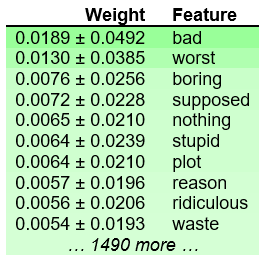
\includegraphics[width=0.7\textwidth]{Bilder/MovieReviews-SentimentClassification_Weights.PNG}
	 \captionof{figure}{Top Features Film Review Klassifizierung}
\end{minipage}\hfill
\begin{minipage}[t]{0.45\linewidth}
\vspace{20pt}
Bei einer binären Klassifizierung verhält sich ELI5  so dass nur eine Klasse (in diesem Fall `neg') dargestellt wird. Die Farbe Grün stellt immer die aktuell gewählte Klasse dar weshalb hier in diesem Beispiel auch negative Wörter grün eingefärbt sind.
\end{minipage}
\end{center}

Um den Text eines Datensatzes zu visualisieren verwendet man die Methode ``explain\_prediction()'', welche sowohl den Einfluss der Features als auch eine Darstellung des Textes mit den hervorgehobenen Schlüsselwörtern anzeigt. Je nach verwendetem Modell weicht die Darstellung von dem hier dargestellten Bild ab, bei gewissen Tree Algorithmen (z.Bsp. DecisionTree) wird zusätzlich noch die Baumstruktur angezeigt.

\parag{Positive Klassifikation - Eintrag 413}
Der erste Datensatz ist eine positive Kritik über den Film ``The Perfect Storm''.
\begin{lstlisting}[language=Python]
doc = documents[413]
eli5.explain_prediction(classifier, doc, vec=vectorizer,target_names=['neg','pos'], top=20)
\end{lstlisting}
\label{eli5413}

\begin{center}
\begin{minipage}[t]{\linewidth}
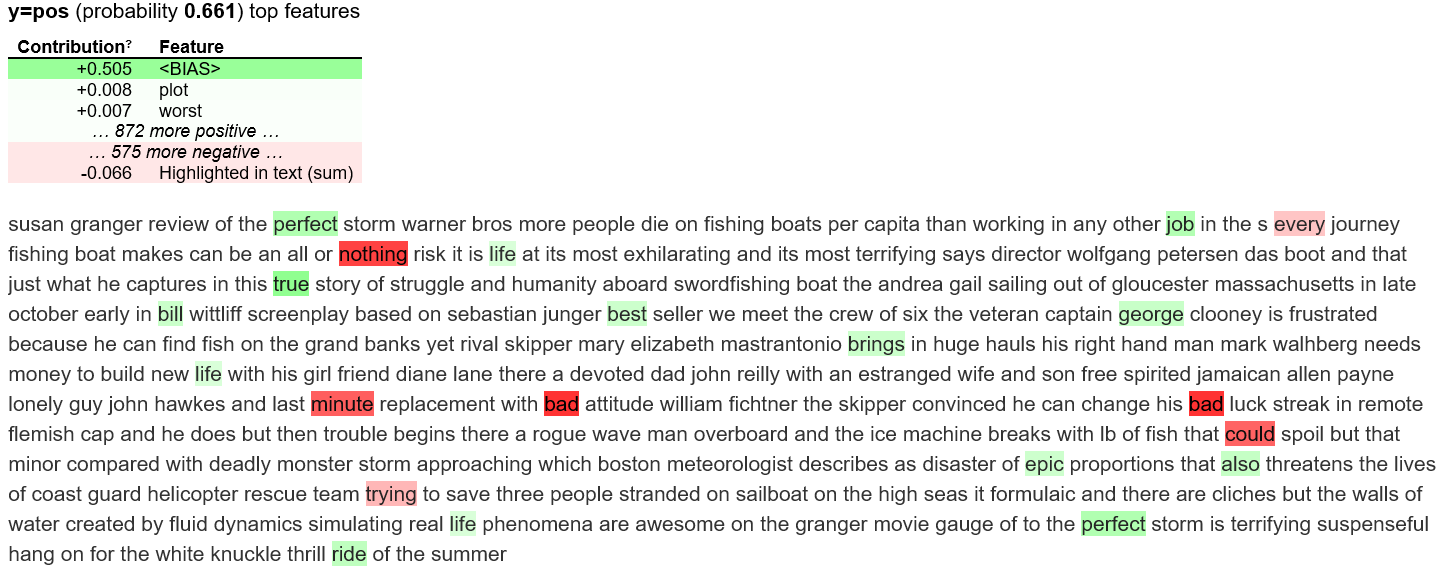
\includegraphics[width=\textwidth]{Bilder/MovieReviews-SentimentClassification_ELI5-413.PNG}
\captionof{figure}{Visualisierung positives Film Review mit ELI5}
\end{minipage}
\end{center}

Mit 66\% Wahrscheinlichkeit für die Klasse ``pos'' ist die Einschätzung für diese Klasse eher tief. Der grösste Anteil an der Klassifizierung haben Features welche ELI5 nicht als Wörter im Text gefunden hat, deshalb ist der Eintrag ``<BIAS>'' an erster Stelle der Feature Tabelle. Auf den ersten Blick stechen die negativen Einflüsse wie ``bad'' und ``nothing'' hervor. Insgesamt überwiegen jedoch die positiv eingeschätzten Wörter in der Summe.

\parag{Negative Klassifikation - Eintrag 414}
Der zweite Beitrag stammt aus dem Datensatz mit den als negativ eingeschätzten Kritiken.
\begin{lstlisting}[language=Python]
doc = documents[414]
eli5.explain_prediction(classifier, doc, vec=vectorizer,target_names=['neg','pos'], top=20)
\end{lstlisting}
\label{eli5414}
Dieser Text wurde mit 83\% klar als ``neg'' klassifiziert.
\begin{center}
\begin{minipage}[t]{\linewidth}
	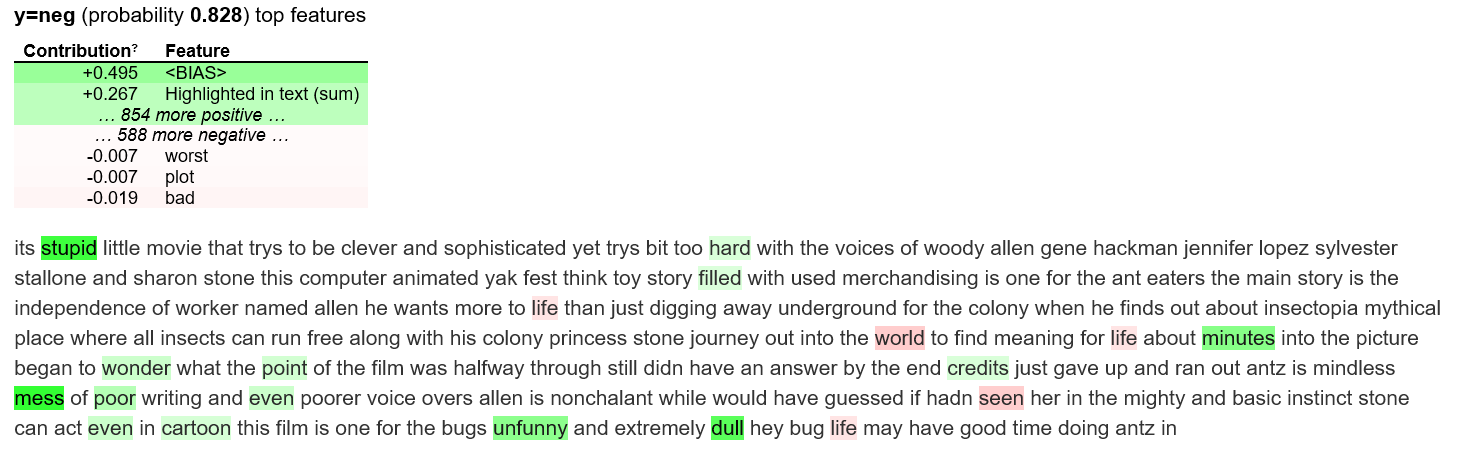
\includegraphics[width=\textwidth]{Bilder/MovieReviews-SentimentClassification_ELI5-414.PNG}
	\captionof{figure}{Visualisierung negatives Film Review mit ELI5}
\end{minipage}
\end{center}
Bei der Darstellung des negativen Film Reviews fällt auf dass Wörter, welche für eine negative Stimmung stehen, Grün markiert sind. Dies kommt daher dass für ELI5 die wahrscheinlichste Klasse `neg' ist mit 81\% Wahrscheinlichkeit und deshalb alle Schlüsselwörter welche auf diese Klasse hinweisen grün markiert werden. In diesem Fall konnte die erzeugte Erklärung immer noch den grössten Anteil nicht visualisieren (``<BIAS>'' mit 0.495 Prozentpunkten) aber die hervorgehobenen Wörter zeigen 

\subsubsection*{Visualisierung durch LIME}
Eine zweite Bibliothek um Visualisierte Erklärungen zu generieren ist \parencite{lime}. Wie der Name andeutet verwendet diese Bibliothek die Technik \Gls{limeG} um aus einem beliebigen Modell Erklärungen zu erzeugen. Der Aufbau des Versuches ist gleich wie vorher mit ELI5, die Daten und das Text Pre-Processing sind identisch. Der Source Code kann hier \cite{textClassLime} heruntergeladen werden.

\parag{Positive Klassifikation - Eintrag 413}
Da das gleiche Modell verwendet wird ist die Wahrscheinlichkeit für die Klasse ``pos'' immer noch 66\%.
\imgText{MovieReview-RandomForest-Display-413.PNG}{Visualisierung positives Film Review mit LIME}{
Die meisten der hervorgehobenen Wörter entsprechen der Visualisierung mit ELI5, eine Ausnahme bildet das Wort ``nothing'' welches durch ELI5 als starker Einfluss für die Klassifikation ``neg'' identifiziert wurde. Auch fällt auf dass das Wort ``bad'' durch ELI5 stark negativ gewichtet wurde währen mit LIME das Wort sogar leicht positiv gewichtet wird.
}

\parag{Negative Klassifikation - Eintrag 414}
Ebenso wie die positive Kritik wird nun auch die negative Kritik mit dem selben Modell visualisiert.
\imgText{MovieReview-RandomForest-Display-414.PNG}{Visualisierung negatives Film Review mit LIME}{
Die negative Kritik entspricht in der Visualisierung der Darstellung mit ELI5. Im Gegensatz zu der positiven Kritik fallen hier keine Unterschiede in der Gewichtung auf.
}

\parag{Fazit Vergleich ELI5 und LIME}
Wie sich gezeigt hat können kleine Unterschiede zwischen den Erklärungen verschiedener Techniken auftreten. Dies ist nicht weiter verwunderlich da \Gls{limeG} mit generierten Modellen arbeitet welche eine Annäherung an das zu beobachtende Modell darstellen. Grundsätzlich sind die Erklärungen aber vergleichbar.

\parag{Versuch 3: Naive Bayes Klassifikator}
Als letzter Versuch wird noch ein Klassifikator mit dem \Gls{nb} Algorithmus welcher bereits in \ref{nb} beschrieben wurde untersucht.
\begin{lstlisting}
from sklearn.naive_bayes import MultinomialNB
classifierNB = MultinomialNB().fit(X_train, y_train)
\end{lstlisting}

\imgText{MovieReview-NB-Accuracy.PNG}{Konfusionsmatrix, Test Zusammenfassung und Accuracy für Naive Bayses}{
Dieser Klassifikator hat eine etwas geringere Accuray als der RandomForest Klassifikator mit einer Accuracy von 0.8. Diese ist aber immer noch weit besser als mit dem einfachen \Gls{DT} Algorithmus.
}
Wie zu erwarten unterscheidet sich die Darstellung etwas von den vorherigen. Da aber ein anderes Modell verwendet wurde ist dies nicht erstaunlich.
\begin{center}
    \begin{minipage}[t]{0.45\textwidth}
    		\vspace{0pt}
		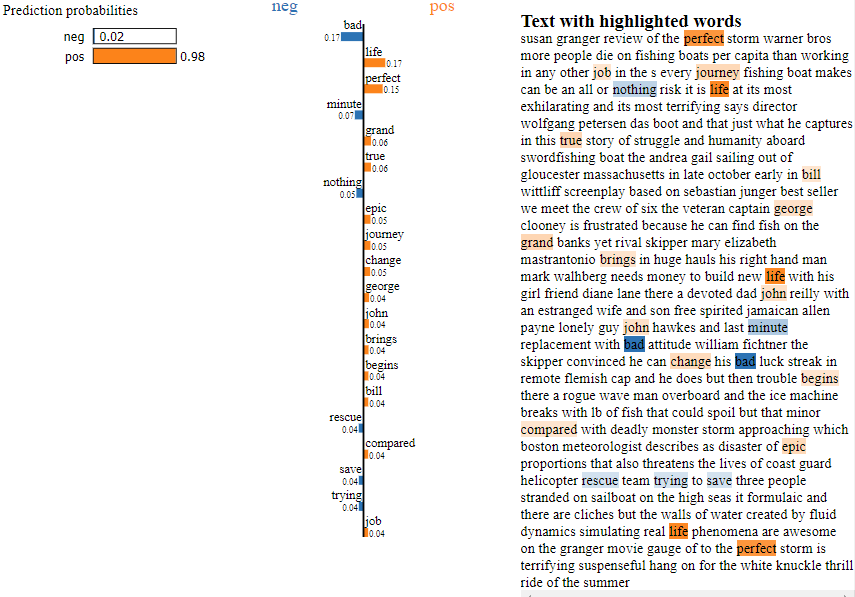
\includegraphics[width=\textwidth, left]{Bilder/MovieReview-NaiveBayes-Display-413.PNG}
		\captionof{figure}{Visualisierung positives Film Review mit LIME und NB}
	\end{minipage}\hfill
    \begin{minipage}[t]{0.45\textwidth}
    		\vspace{0pt}
  		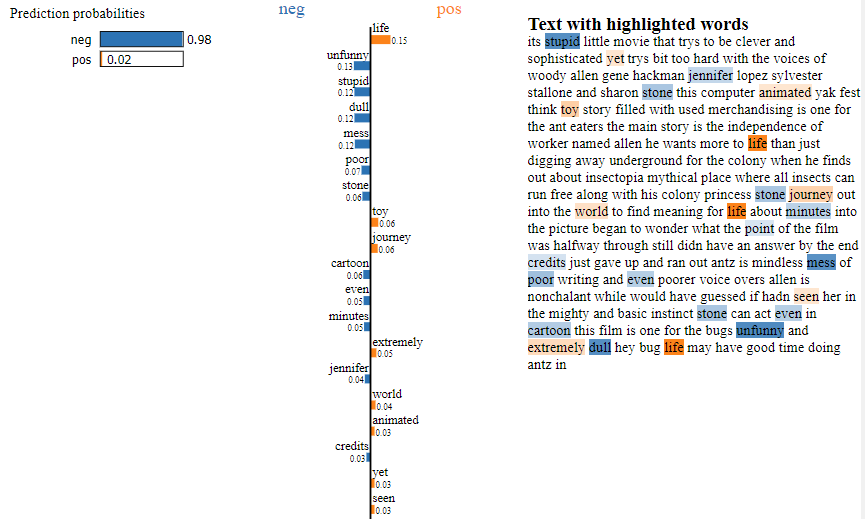
\includegraphics[width=\textwidth, left]{Bilder/MovieReview-NaiveBayes-Display-414.PNG}
		\captionof{figure}{Visualisierung negatives Film Review mit LIME und NB}
    \end{minipage}
\end{center}

\parag{Fazit}
Auch unterschiedliche Klassifikations-Algorithmen können einfach dargestellt und verglichen werden. Dadurch können Auffälligkeiten leicht entdeckt werden und Anpassungen (andere Algorithmen, geändertes Pre-Processing usw.) getestet werden. 

\subsection{Black Box Modell}
Während in dem vorherigen Beispiel ein \Gls{Whitebox} Modelle mit interpretierbaren Algorithmen angewendet wurde, können auch \Gls{Blackbox} Modelle analysiert werden. Dafür benutzen sowohl \cite{ELI5} als auch \cite{lime} das \acrshort{lime} Verfahren um die Vorhersage zu erklären und das Modell zu interpretieren.

\parag{Daten}
Der selbe Datensatz wie in \ref{eli5MovieReview} wurde für einen weiteren Klassifikator genutzt, dieses Mal allerdings mit dem \acrfull{lstm} Verfahren welches zu den neuronalen Netzen gehört. 

\parag{Verwendete Bibliotheken}
Die Grundlage des Skriptes bildet der Blog-Beitrag \parencite{nThLIME} welcher für die geänderte Datenquelle angepasst wurde. 
Das Experiment verwendet \cite{nltk} um die Texte vorzubereiten, scikit-learn \cite{scikit-learnLink} und Tensorflow \cite{TensorFlow} für die Klassifikation und \cite{ELI5} um aus den Ergebnissen Erklärungen zu generieren. 


\subsubsection*{Visualisierung eines LSTM  mit LIME}
Das Jupyter Notebook mit dem gesamten Source Code ist auf github.com vorhanden \parencite{textClassLSTM}.
 
 Das neuronale Netz ist sehr einfach gehalten um die Trainingszeit kurz zu halten. Es handelt sich hier um einen Klassifikator des Typs \Gls{binClassificator} wie man an dem letzten Layer mit nur einem Ausgang sieht.
\begin{lstlisting}[language=Python, caption=LSTM Modell für LIME Movie Sentiment Analyse]
model = Sequential()
model.add(Embedding(max_features, 128))
model.add(Bidirectional(LSTM(128, dropout=0.5, recurrent_dropout=0.5)))
model.add(Dense(1, activation='sigmoid'))
model.compile('adam', 'binary_crossentropy', metrics=['accuracy'])
\end{lstlisting}

In 8 Durchgängen wird das Netz trainiert, als Wrapper für Tensorflow dient hier Keras, die Vorbereitung der Daten übernimmt eine scikit-learn Pipeline.
\begin{lstlisting}
sklearn_lstm = KerasClassifier(build_fn=create_model, epochs=8, batch_size=batch_size, max_features=max_features, verbose=1)

# Build the Scikit-learn pipeline
pipeline = make_pipeline(sequencer, padder, sklearn_lstm)

pipeline.fit(texts_train, y_train)
\end{lstlisting}

\begin{center}
    \begin{minipage}[t]{0.45\textwidth}
    		\vspace{0pt}
		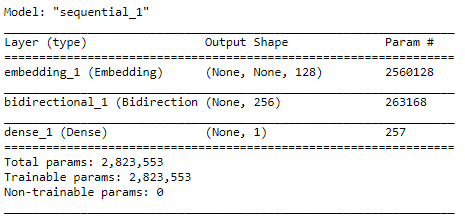
\includegraphics[width=\textwidth, left]{Bilder/MovieReview-LSTM-Summary.PNG}
		\captionof{figure}{Zusammenfassung LSTM Netz für Movie Sentiment Analyse}
	\end{minipage}\hfill
    \begin{minipage}[t]{0.45\textwidth}
    		\vspace{0pt}
  		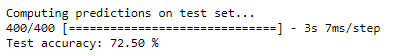
\includegraphics[width=\textwidth, left]{Bilder/MovieReview-LSTM-Accuracy.PNG}
		\captionof{figure}{Performance des LSTM Netz für Movie Sentiment Analyse}
    \end{minipage}
\end{center}
Die Qualität der Klassifizierungen liegt tiefer als bei den vorherigen Beispielen mit dem RandomForest und dem Naive Bayes Klassifikator. Dies ist bei einem solch einfach aufgebautem neuronalen Netz nicht erstaunlich.
\parag{Positive Klassifikation - Eintrag 413}
Erneut wird der bereits vorher in \ref{eli5413} positiv klassifizierte Beitrag mit der Id 413 analysiert.
\begin{lstlisting}
Probability(positive) = 0.99591535
True class: positive
\end{lstlisting}
Das Resultat ist fällt für dieses Modell eindeutig aus: 99\% Wahrscheinlichkeit für die Klasse ``positiv''.
\imgText{MovieReview-LSTM-Display-413.PNG}{Visualisierung Movie Review 413}{
Obwohl die Klassifizierung auch diesmal positiv ist werden völlig andere Wörter für dieses Resultat verantwortlich gemacht.
Auffallend ist dass das Wort ``bad'' für dieses Modell in diesem Text keine Relevanz hat. Auch die restliche Liste der relevanten Wörter ist fast vollständig verschieden von allen anderen Modellen die bereits untersucht wurden.
}

\parag{Negative Klassifikation - Eintrag 414}
Auch dieser Text wird korrekt als ``negativ'' klassifiziert, auch hier mit einer hohen Wahrscheinlichkeit von 96\%.
Auch der Eintrag 414 wird wie bereits in \ref{eli5414} analysiert.
\begin{lstlisting}
Probability(positive) = 0.037772316
True class: negative
\end{lstlisting}
\imgText{MovieReview-LSTM-Display-414.PNG}{Visualisierung Movie Review 414}{
Das Wort ``unfunny'' wurde wie auch in der ersten Analyse als stark relevant für die Klassifikation befunden während diesmal ``stupid'' keine Beachtung findet. Ein Fehler in der Vorbereitung der Texte wird durch diese Darstellung deutlich sichtbar: Die Filterung der Stopp-Wörter scheint nicht korrekt zu funktionieren, die beiden Wörter ``and'' und ``in'' sollten nicht in die Klassifizierung mit einbezogen werden.
}

\parag{Fazit}
Auch das Erklären von neuronalen Netzen

\chapter{Schwächen von Modellen erkennen}
\label{vulnearabilities}

Die in den vorherigen Kapiteln vorgestellten Techniken erlauben einen besseren Einblick in die Funktionsweise von \glsentrylong{ML} Modellen. Dieses Wissen kann dazu genutzt werden um Schwächen oder auch gezielte Angriffe auf Anwendungen mit integrierten \Gls{ML} Modellen zu erkennen.

\section{Diskriminierung durch Bias}
Als \Gls{BIAS} werden Tendenzen bezeichnet, welche in Modellen vorhanden sind und durch nicht ausgewogene Trainingsdaten erzeugt werden.
Ein bekanntes Beispiel dazu ist ein Chat-Bot, welcher von Microsoft entwickelt wurde und der sein Verhalten durch Twitter Tweets trainierte. Das Experiment musste von Microsoft nach kurzer Zeit abgebrochen werden, da der Chat-Bot eine Tendenz zu rassistischen und beleidigenden Antworten hatte. Verursacht wurde dieses Verhalten durch gezielte Manipulationen durch andere Twitter Benutzer, die eine Gelegenheit sahen den Chat-Bot auszutricksen. Eine Beschreibung der Probleme dieses Projektes wurde in dem Artikel \parencite{msTay} dokumentiert.
Dieser Fall kann auch als Beispiel für ``Data Poisoning'' angesehen werden, da die Lerndaten des Bots gezielt beeinflusst wurden, siehe \ref{dataP}.

\section{Manipulierte Bilder: Adversarial Attacks}
\label{Adversarial Attacks}
Wie bereits in Kapitel \ref{Sicherheit} angedeutet, sind \Gls{ML} Anwendungen oftmals unerwartet empfindlich auf kleinste Änderungen an den Eingangsdaten. In einer Arbeit von Google Forschern   \parencite{Goodfellow2014} konnte gezeigt werden dass dies eine grundsätzliche Eigenschaft nicht nur von neuronalen Netzen, sondern auch anderen linearen Klassifikatoren ist. Erklärbar ist ein solches Fehlverhalten wenn man sich vor Augen hält, dass neuronale Netze und andere Klassifikatoren keine abstrakten Konzepte wie ``Tier'' oder auch ``Fahrzeug'' lernen, sondern sich alleine an den für das Training verwendeten Bilddaten orientieren.

\imgText{adversarial.png}{Adversarial Beispiel \protect\footnotemark{}}{
Ein Beispiel für die Manipulation eines Bildklassifikators stammt aus der Arbeit ``Intriguing properties of neural networks'' \parencite{Szegedy2013}. 
\break\break
Die linke Spalte zeigt ein korrekt klassifiziertes Bild.
\break\break
Die mittlere Spalte stellt den Unterschied zwischen dem korrekt klassifizierten Bild und der falschen Klasse dar.
\break\break
Rechts ist das mit der Adversarial Technik manipulierte Bild zu sehen.
\break\break
Alle Bilder in der Rechten Spalte wurden als ``Ostrich'' (Strauss) klassifiziert!
}
\footnotetext[1]{Quelle: Szegedy  \parencite{Szegedy2013}}

\parag{Adversarial Attacken selber erzeugen}
Die Tensorflow Webseite stellt ein Tutorial zu Verfügung, das die Erzeugung solcher ``Adversarial'' Bilder erläutert: \parencite{tensorflowFGSM}

Eines der in dem Tutorial erzeugten Bilder wird schliesslich als ``brain coral'' (Hirnkoralle) erkannt, allerdings mit deutlich sichtbaren Bild-Artefakten. Für das menschliche Auge sieht es jedoch aus als ob das Bild stark verrauscht wäre und nicht nach einem gezielt manipulierten Bild.
\begin{center}
\begin{minipage}[t]{0.45\linewidth}
	\vspace{0pt}
	\centering
	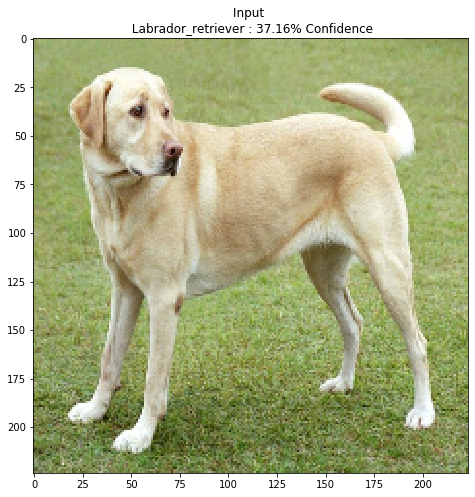
\includegraphics[width=0.9\textwidth]{Bilder/tensorflow-adversarial-original.png}
	 \captionof{figure}{Ursprungs-Bild\protect\footnotemark{}}
\end{minipage}\hfill
\begin{minipage}[t]{0.45\linewidth}
	\vspace{0pt}
	\centering
	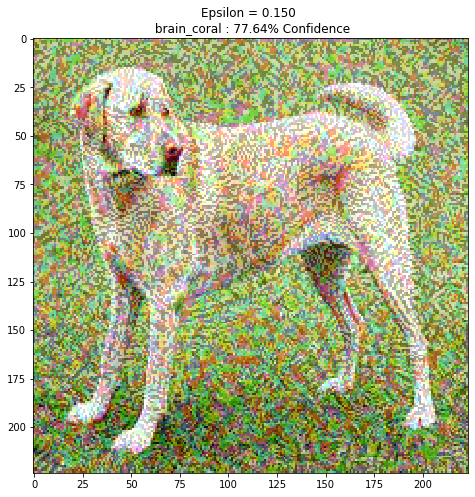
\includegraphics[width=0.9\textwidth]{Bilder/tensorflow-adversarial-fake.png}
	 \captionof{figure}{Durch Adversarial Angriff erzeugtes Bild}
\end{minipage}
\end{center}
\footnotetext[2]{Quelle: \parencite{tensorflowFGSM}}

\subsubsection*{Täuschung der Verkehrszeichen-Erkennung eines Tesla}
Ein interessantes Beispiel einer solchen ``Adversarial Attack'' ist die Arbeit eines Teams von McAffe Labs, welches gezielt das System eines Tesla angegriffen hat. Schlussendlich wurde das Auto dazu gebracht anstatt 35mph (ca. 55kmh)  85mph (ca. 135kmh) als Geschwindigkeitsbegrenzung zu erkennen.

\parencite{advTesla} 

\begin{center}
\begin{minipage}[t]{0.45\linewidth}
	\vspace{0pt}
	\centering
	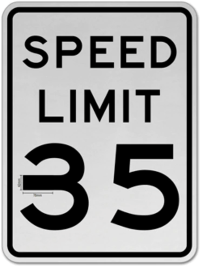
\includegraphics[width=0.7\textwidth]{Bilder/speed-limit-fake-small.png}
	 \captionof{figure}{Gefälschtes Verkehrsschild als Adversarial Attack\protect\footnotemark{}}
\end{minipage}\hfill
\begin{minipage}[t]{0.45\linewidth}
	\vspace{0pt}
	Eine Verlängerung des mittleren Balkens einer Drei führte das neuronale Netz eines Tesla zu einer Fehlklassifizierung als Acht und dadurch zu einer erlaubten Geschwindigkeit von 85 Meilen pro Stunde. Obwohl die veränderte Ziffer durchaus an eine Acht erinnern kann, sehen Menschen die Ziffer trotzdem als Drei, im Gegensatz zu den Systemen des Teslas.
\break\break
Mittlerweile wurde das Verhalten der Tesla-Systeme angepasst und diese spezifische Attacke ist nun nicht mehr möglich.
\end{minipage}
\end{center}
\footnotetext{Quelle: \parencite{advTesla}}

\subsubsection*{Eigene Versuche mit Adversarial Attacks}
Durch die Arbeit einiger Forscher \parencite{papernot2018cleverhans} gibt es eine Python Bibliothek \parencite{cleverHans}, welche die Erzeugung von Adversarial Angriffen erleichtert.

\section{Manipulierte Daten: Data Poisoning}
\label{dataP}
Mit ``Data Poisoning `` werden Techniken benannt, die \Gls{ML} Modelle über die Trainingsdaten angreifen. Oftmals werden Modelle nach einem initialen Training mit einem festen Datensatz wiederkehrend mit aktualisierten Daten erneut trainiert. Ein typisches Beispiel sind Spam Filter die in regelmässigen Intervallen Emails, welche durch die Benutzer als Spam markiert wurden, in ihren Trainingsdatensatz integrieren.
 
Grundsätzlich wird zwischen zwei Arten von Data Poisoning unterschieden:
\begin{description}
  		\item[Availability] Das Ziel einer solchen Attacke ist es die Datenbasis eines \Gls{ML} Modells so zu erweitern, dass die Wahrscheinlichkeit für eine bestimmte Klassifikation entweder stark erhöht oder verringert wird. Wie durch die Arbeit ``Online Data Poisoning Attacks'' \parencite{Zhang2019} nachgewiesen wurde, kann ein solcher Angriff sowohl für überwachtes Lernen wie auch unüberwachtes Lernen erfolgreich eingesetzt werden. 
  		\item[Backdoor Attacks] Ein Backdoor Angriff versucht die Eingangsparameter eines \Gls{ML} Modells so zu wählen, dass ein bestimmtes Ergebnis garantiert ist. Damit kann ein schädliches Programm, welches eigentlich durch einen Virenscanner abgewehrt werden sollte, durch Verwendung einer bestimmten Zeichenkette ungehindert aktiviert werden.\\
  		Es besteht zudem die Möglichkeit, dass ein Modell, welches aus einer externen Quelle bezogen wurde, mit einer ``Backdoor'' ausgestattet ist um auf bestimmte Parameter zu reagieren. In der Arbeit ``BadNets: Evaluating Backdooring Attacks
on Deep Neural Networks'' \parencite{Gu2019} konnte gezeigt werden wie ein \gls{NN} durch bestimmte Aufkleber dazu gebracht werden konnte Stopp-Schilder mit Geschwindigkeitsbegrenzungs-Schildern zu verwechseln.
	\end{description}

\chapter{Fazit}
Das Ziel dieser Arbeit, einen Überblick über den Stand der \Gls{xai} Entwicklung zu bieten, stand vor einem zuerst nicht erwarteten Problem. Die Menge an Methoden, Artikeln und Forschungsarbeiten zu diesem Thema ist sehr gross. Die Entscheidungen welche Methoden erklärt, oder zumindest erwähnt, werden sollten war nicht einfach. Schlussendlich war der experimentelle Teil ausschlaggebend. Einige der Methoden wie \acrshort{svcca} oder \acrshort{tcav} stellten sich als sehr Aufwändig heraus so dass bei einer Wahl eines dieser Themen viele andere Bereiche nicht hätten beachtet werden können.

Der praktische Teil der Arbeit hatte mit einigen Problemen zu kämpfen. Es stellte sich heraus das einige \Gls{xai} Frameworks für Python spezifische Anforderungen an die dem Modell zugrunde liegenden \Gls{ML} Frameworks stellen. Dies ist nicht weiter erstaunlich wenn man bedenkt, dass die Analyse eines Modells tiefer auf die einzelnen Funktionen und Parameter eingehen muss als dies Vorhersagen tun. Das fragile Gleichgewicht der installierten Framework Versionen wurde immer wieder durch die Installation eines weiteren Werkzeuges zunichte gemacht welches eine andere Version von Tensorflow oder Keras benötigte. Eine Erkenntnis ist daher immer mit einer eigenen Umgebung für jedes Projekt zu arbeiten. Anaconda hilft dabei sehr diese Umgebungen zu verwalten. Da aber nicht alle getesteten Bibliotheken in Anaconda vorhanden sind habe ich leider anfangs fehlende Bestandteile über den Python Packetmanager pip installiert. Diese Vorgehensweise war sehr ungünstig und hat mir mehrere Male die Umgebungen mit nicht miteinander kompatiblen Bibliotheksversionen ``verseucht''. Eine saubere Vorgehensweise mit voneinander getrennten Umgebungen ist unbedingt nötig wenn man möchte das Programme auch nach einigen Wochen noch wie gewünscht funktionieren.

Die Auswertung der Ergebnisse durch exploratives Vorgehen war zu Beginn nicht Erfolgreich. Es ist zwar einfach durch Visualisierungen zu erkennen welche Bestandteile eines Bildes für ein neuronales Netz wichtig sind, Schlussfolgerungen daraus zu ziehen stellte sich jedoch als überraschend schwierig heraus. Bei einem direkten Vergleich zwischen verschiedenen Methoden waren oftmals grosse Unterschiede erkennbar was die wichtigen Bestandteile eines Bildes betrifft. Da einige Methoden unter gewissen Umständen nicht funktionieren (Gradient basierte Verfahren haben nachgewiesene Schwächen) steht immer die Frage im Raum ob die Unterschiede zwischen den Visualisierungen von Bedeutung sind. Der zweite Ansatz welcher mit einem konkreten Ziel, nämlich dem Nachweis eines Kluger-Hans Effektes, gestartet war funktionierte bedeutend besser. Die Visualisierung zeigte sehr deutlich welchen Defekt das neuronale Netz hat und könnte in der Realität auch direkt zu einer Verbesserung (durch Anpassung des Trainings- und Testdaten) des Modells führen. Aber auch hier war nur eine von drei eingesetzten Methoden erfolgreich. Dies führt zu einer weiteren Erkenntnis: Jede Analyse sollte mit mehreren Methoden durchgeführt werden.

\chapter{Ausblick}
Die Weiterentwicklung der Methoden von \Gls{xai} sind eng an die zukünftige Entwicklung von \Gls{ML} gekoppelt. Obwohl Prognosen für die Zukunft natürlich schwierig sind, ist es aber momentan wahrscheinlich, dass die grossen Investitionen in \Gls{AI} und \Gls{ML} zumindest noch einige Jahre weitergeführt werden. Durch die Verfügbarkeit von Budgets in Forschung und Industrie, gekoppelt mit den Forderungen vieler Akteure nach einer ``verständlichen'' \Gls{AI}, ist weiterhin mit einer Vielzahl an Arbeiten im Bereich \Gls{xai} zu rechnen. Wie schnell dabei Fortschritte erzielt werden können, ist jedoch völlig ungewiss und die Geschichte der \Gls{AI} zeigt, dass man dabei eine gewisse Vorsicht an den Tag legen sollte.

\section{Aktuelle Probleme}
Obwohl bereits einige Methoden existieren, steht \Gls{xai} immer noch am Anfang seiner Entwicklung. Viele der geforderten Leistungen  sind noch ausstehend oder erst unzureichend erfüllt. Selbst elementare Definitionen sind nicht vorhanden oder werden von Anwendern und Forschern unterschiedlich interpretiert.  

Auch die Qualität der Erklärung ist allgemein eher klein. Die meisten Erklärungen, die durch aktuelle Algorithmen erzeugt werden, können nur Details beschreiben. Es ist zwar gut möglich den Einfluss eines einzelnen Pixels zu berechnen, es besteht jedoch keine Verbindung zu abstrakten Begriffen wie Objekten, Körpern oder Personen. Den erzeugten Erklärungen fehlt es oft an Aussagekraft.

\section{Wünschenswerte Entwicklungen}

\subsection{Mathematisch begründete XAI}
\Gls{xai} benötigt nach Samek \parencite{Samek2019a} eine formale und allgemein akzeptierte Definition was Erklärungen genau sind.
Ein möglicher Weg für eine mathematische Begründung einer Erklärung zeigt die Arbeit von Montavon \parencite{Montavon2017} durch die Integration der Taylor decomposition.

\subsection{Modell agnostische Methoden}
Wie sich auch in dieser Arbeit gezeigt hat, sind \acrshort{XAI} Implementierungen der XAI Werkzeuge schwierig anzuwenden. Oftmals müssen die Modelle bestimmte Bedingungen erfüllen damit eine Analyse möglich ist. In anderen Fällen konnte keine funktionierende Erklärung erzeugt werden, ohne dass man herausfinden konnte weshalb. Weitere Algorithmen wie \acrshort{lime}, welche allgemein funktionieren, sind nötig. Ein grosser Fortschritt wäre eine allgemein anwendbare Erklärungsfunktion, ähnlich wie Keras bereits eine Abstraktion für \Gls{ML} Implementierungen bereitgestellt hat. 

\subsection{Automatisierung}
Für die Zukunft wäre es wünschenswert, wenn allgemeine Regeln automatisiert geprüft werden könnten. Mögliche Aufgaben wären dabei die Suche nach einem eventuell vorhandenen \Gls{BIAS} oder die Anfälligkeit auf Angriffe wie \acrlong{aip} oder Data Poisoning.

\section{Fehlende Lösungen}
Es besteht die Möglichkeit dass die hohen Erwartungen an \Gls{xai} nicht erfüllt werden, sie es weil es sich als Unmöglich herausstellt die Vorhersagen in der gewünschten, für Menschen verständlichen, Abstraktion zu erzeugen. Oder die Qualität der Vorhersagen wird nicht erreicht da die Diskrepanz zu dem realen Modell zu hoch bleibt. Falls dieses Szenario eintritt 
\parencite{Rudin2018}

\chapter{Anhang}
\section{Source Code}
\label{dt-vis}

\subsection{Entscheidungsbaum Visualisierung mit sklearn und Graphviz}
Der folgende Code benötigt mindestens scikit-learn 0.22.
\begin{lstlisting}[language=Python, caption=Decision Tree Visualisierung]
from sklearn.datasets import load_iris
from sklearn import tree
from sklearn import datasets

X, y = load_iris(return_X_y=True)
clf = tree.DecisionTreeClassifier()
clf = clf.fit(X, y)

iris = datasets.load_iris()

dot_data = tree.export_graphviz(clf, out_file=None, 
                      feature_names=iris.feature_names,  
                      class_names=iris.target_names,  
                      filled=True, rounded=True,  
                      special_characters=True)  

# print tree as text
from sklearn.tree import export_text
r = export_text(clf, feature_names=iris['feature_names'])
print(r)

# print tree as colored top-down tree
import graphviz
graph = graphviz.Source(dot_data)  
graph 

# plot decision surface
import numpy as np
import matplotlib.pyplot as plt
# Parameters
n_classes = 3
plot_colors = "ryb"
plot_step = 0.02

for pairidx, pair in enumerate([[0, 1], [0, 2], [0, 3],
                                [1, 2], [1, 3], [2, 3]]):
    # We only take the two corresponding features
    X = iris.data[:, pair]
    y = iris.target
    
    # Train
    dTree = tree.DecisionTreeClassifier().fit(X, y)

    # Plot the decision boundary
    plt.subplot(2, 3, pairidx + 1)

    x_min, x_max = X[:, 0].min() - 1, X[:, 0].max() + 1
    y_min, y_max = X[:, 1].min() - 1, X[:, 1].max() + 1
    xx, yy = np.meshgrid(np.arange(x_min, x_max, plot_step),
                         np.arange(y_min, y_max, plot_step))
    plt.tight_layout(h_pad=0.5, w_pad=0.5, pad=2.5)

    Z = dTree.predict(np.c_[xx.ravel(), yy.ravel()])
    Z = Z.reshape(xx.shape)
    cs = plt.contourf(xx, yy, Z, cmap=plt.cm.RdYlBu)

    plt.xlabel(iris.feature_names[pair[0]])
    plt.ylabel(iris.feature_names[pair[1]])

    # Plot the training points
    for i, color in zip(range(n_classes), plot_colors):
        idx = np.where(y == i)
        plt.scatter(X[idx, 0], X[idx, 1], c=color, label=iris.target_names[i],
                    cmap=plt.cm.RdYlBu, edgecolor='black', s=15)

plt.suptitle("Decision surface of a decision tree using paired features")
plt.legend(loc='lower right', borderpad=0, handletextpad=0)
plt.axis("tight")
\end{lstlisting}
https://scikit-learn.org/stable/modules/tree.html

\subsection{Bild-Klassifikation mit tf-explain}
Das folgende Programm erzeugt mit den Bibliotheken Tensorflow (2.0) und tf-explain und en Algorithmen ``Grad CAM'' und ``Integrated Gradients'' Visualisierungen einer Bild-Klassifizierung. 
\begin{lstlisting}[language=Python, caption=Visualisiertes Neuronales Netz mit Tensorflow und tf-explain]
import tensorflow as tf
from keras.applications.vgg16 import VGG16
from keras.preprocessing.image import load_img
from keras.preprocessing.image import img_to_array
from keras.applications.vgg16 import preprocess_input
from keras.applications.vgg16 import decode_predictions

model = tf.keras.applications.vgg16.VGG16(weights="imagenet", include_top=True)

#print(model.summary())

imageOrig = load_img('D:/Master Thesis/dogs-vs-cats/test/DSC05797.JPG', target_size=(224, 224))
imageArr = img_to_array(imageOrig)  #output Numpy-array

imageReshaped = imageArr.reshape((1, imageArr.shape[0], imageArr.shape[1], imageArr.shape[2]))

image = preprocess_input(imageReshaped)
predictions = model.predict(imageReshaped)

import numpy as np
top5predictions = np.argsort(predictions)[0,::-1][:5]

labels = decode_predictions(predictions)

for label in labels[0]:
    print('%s (%.2f%%)' % (label[1], label[2]*100))
    
from tf_explain.core.grad_cam import GradCAM
from mpl_toolkits.axes_grid1 import ImageGrid

def createImageGrid(imageOrig, predictions, labels, explainer, explainerArgs):
    camImages = [imageOrig]
    fig = plt.figure(figsize=(20., 20.))
    grid = ImageGrid(fig, 111,  # similar to subplot(111)
                 nrows_ncols=(2, 3),
                 axes_pad=0.5,  # pad between axes in inch.
                 )
    for class_index in top5predictions:
        camImages.append(explainer.explain(class_index=class_index, **explainerArgs))
    
    i = -1
    for ax, im in zip(grid, camImages):
        # Iterating over the grid returns the Axes.
        ax.set_xticks([])
        ax.set_yticks([])
        label = labels[0][i]
        if i >= 0:
            ax.set_title('%s (%.2f%%)' % (label[1], label[2]*100), fontsize=20)
        ax.imshow(im)
        i = i + 1

    plt.show()


explainer = GradCAM()
createImageGrid(imageOrig, predictions, labels, explainer, {'model': model, 'layer_name': 'block5_conv3', 'validation_data': data})

from tf_explain.core.gradients_inputs import GradientsInputs
explainer = GradientsInputs()
createImageGrid(imageOrig, predictions, labels, explainer, {'model': model, 'validation_data': (np.array([imageArr]), None)})

from tf_explain.core.integrated_gradients import IntegratedGradients

explainer = IntegratedGradients()
createImageGrid(imageOrig, predictions, labels, explainer, {'model': model, 'validation_data': (np.array([imageArr]), None)})
\end{lstlisting}
https://github.com/sicara/tf-explain

\subsection{Visualisierung einer Klassifikation mit lime}
Die Visualisierung mit lime benutzt als Grundlage das Tutorial ``Image Classification Kears'' \parencite{limeKeras}.
\begin{lstlisting}[language=Python, caption=Visualisiertes Neuronales Netz mit Tensorflow und lime]
import lime 
from lime import lime_image

explainer = lime_image.LimeImageExplainer()


explanation = explainer.explain_instance(np.vstack([imageArr]), model.predict, top_labels=5, hide_color=0, num_samples=1000)

from skimage.segmentation import mark_boundaries

camImages = [imageOrig]
fig = plt.figure(figsize=(20., 20.))
grid = ImageGrid(fig, 111,  # similar to subplot(111)
             nrows_ncols=(2, 3),
             axes_pad=0.5,  # pad between axes in inch.
             )
for class_index in range(0,5):
    temp, mask = explanation.get_image_and_mask(explanation.top_labels[class_index], positive_only=True, num_features=5, hide_rest=True)
    camImages.append(mark_boundaries(temp / 2 + 0.5, mask))

i = -1
for ax, im in zip(grid, camImages):
    # Iterating over the grid returns the Axes.
    ax.set_xticks([])
    ax.set_yticks([])
    label = labels[0][i]
    if i >= 0:
        ax.set_title('%s (%.2f%%)' % (label[1], label[2]*100))
    ax.imshow(im)
    i = i + 1

plt.show()
\end{lstlisting}

\appendix
% Glossary
\printglossary[type=\acronymtype]
\printglossary[type=main]
% List of Figures
\listoffigures
% List of Tables
\begingroup
\let\clearpage\relax
\listoftables
% Bibliography
\printbibliography[type=article,title={Literaturverzeichnis Artikel}]

\printbibliography[type=book,title={Literaturverzeichnis Bücher}]

\printbibliography[type=misc,title={Linkverzeichnis}]
%Index
\addcontentsline{toc}{chapter}{Index}
%\printindex
% Appendices
\lstlistoflistings
\endgroup

\end{document}
